Back-end developers get no respect. That is unless you’re at a technology-driven company like Atari. David Shepperd was the longest serving of Atari’s programmers and a highly keen technology drive from the earliest days of programming up until the figurative death of the arcade game. He started by creating some of Atari’s most successful, stable hits of the 70s and then moved to creating stable development tools over the rest of his tenure.

Mr. Shepperd remains modest about his work but with a stunning memory capacity which sheds some light on the ins and outs of Atari’s coin-op programming division. This chat takes you on a journey of early computer hobbyist work, the creative interference in the company’s early days, the relationship of Atari Games with Atari Corp, and the grand camaraderie of the folks who saw the industry grow together.

\noindent\makebox[\linewidth]{\rule{\paperwidth}{0.4pt}}

\textcolor{interviewer}{Interviewer:} Tell me about your early career in electronics.

\textcolor{interviewee}{David Shepperd:} I had an interest in electronics from a very early age. My dad bought a correspondence course on electronics when I was very young (maybe 10 or so). He completed the course but never did anything in electronics himself. As part of the course he was given breadboards, components, etc. and had to build a number of working items including a fully functioning oscilloscope. I was mesmerized by all of it and when he was done with all the parts I got to play with them and tried to figure out what was going on. I remember taking the scope to school in 8th grade to show the science class. The kids weren't impressed, but the science teacher was very interested in it. I barely knew what knobs to turn to get a picture on it.

In 10th, 11th, and 12th grades my two optional shop classes were in electronics. Two hours each day of electronics shop; it was cool except much to my dismay we didn't get to learn much electronics. In 12th grade there was some discussion about how transistors worked though. Then in junior college I took more electronics and electrical engineering classes (as many as I could fit in). This was much more interesting, however the instructor was learning the material at the same time as us (he said as much). I loved those classes and did very well in them and the math that had to go with it, although I don't think of myself as much of a math wizard. 

\textcolor{interviewer}{Interviewer:} After that did you get a formal engineering education?

\textcolor{interviewee}{David Shepperd:} I went to a trade school after junior college, DeVry University in Phoenix, Arizona. Again that was focused on EE work. I'd say it was very in depth with lots of hands on lab work too. I also had a well equipped lab in my apartment with lots of junk from junk stores and dumpster diving. I was always tinkering with circuits to do this and that. It probably was mostly with transistors, but I'm pretty sure there were some of the newly minted integrated digital circuits in there too and those must have mostly been from Texas Instruments. 

It was at DeVry I learned all the ins and outs of television and radio. Even though that information was presented in the first couple of quarters it stuck to me and I didn't forget any of it., and I drew on all the knowledge later when I did my own video system. One interesting thing about the video and TV is at school they were very clear to point out the TV signal's specifications: so many microseconds for this and so many milliseconds for that. It led me to believe the TV's required very tight timing on the input television signal. Much later when I designed my video sync chain (that’s what we called the circuit that produced the horizontal and vertical sync signals the TV needed) I adhered to those specs as tightly as I could adding front and back porches, carefully timed pulses, voltage levels, etc. Only after I started at Atari did I learn the TV's don't much give a damn about porches and pulse widths and whatnot, nor are they too critical of voltage levels. They pretty much will sync on anything as long as it is reasonable and show a decent picture as long as the signal is not too far out of whack.

Interviews: How did you first start working as a programmer then?

\textcolor{interviewee}{David Shepperd:} I took a programming class at a junior college in 1968 or 1969. It was a Fortran II class taught on an IBM 1620 (with 20k of core memory!). That set the hook. My college course work was in electrical engineering, working towards a EE (I never got it). 

When I left school in 1972 I took a job in Cupertino, CA in a factory that made 3rd party disk drives that could be plugged into various mainframe and mini-computers from IBM, DEC, UNIVAC and others. These were the big drives the size of a washing machine having 3 kilowatt voice coil hurling 20 heads across 14 inch platters. I think the top end drive held 100MB and cost over \$20k at retail. 

I was hired on as a technician and worked in the factory floor for about 6 months then transferred into the engineering department. Things were very sedate there but they had plenty of high tech machines and test equipment. There was an IBM 360/65, a 360/50, a 370/145 mainframe in the lab, and a myriad of fancy expensive test equipment (all of it usable by me for whatever I wanted to do). They were mainly there to test new engineering designs as they popped up and sat idle all the rest of the time. Lots of opportunity to program different things and in different languages (mainly Fortran IV, 360/370 assembly, and COBOL). I was having a blast.

\textcolor{interviewer}{Interviewer:} How did video games enter the picture for you?

\textcolor{interviewee}{David Shepperd:} Along about 1974 I went to the beach boardwalk in Santa Cruz, California and in an arcade they had one or two video games. I don't remember what games they were, but I'm thinking Computer Space from Nutting Associates might have been one of them that stuck with me. Again, I was hooked, but I was also a cheapskate and knew immediately I would end up putting all my hard earned money into these machines, one quarter at a time. I had learned how TVs worked in school and figured I could cobble together a circuit from parts collected dumpster diving that I could use to draw a picture. 

\begin{tcolorbox}[]
    Computer Space, released in November of 1971, was the pre-Atari video game developed by Nolan Bushnell and Ted Dabney for Nutting Associates in California. It remained the most technologically adept game on the market for several years and inspired a number of Atari game creators.
\end{tcolorbox} 

It took me a few months, but eventually I had something that could draw a single little picture (later known as a sprite) on the screen of an old 12 inch black and white TV I had and I could move the picture around with a couple of buttons. No sooner had I finished that when I went back to the boardwalk only to discover a game from Atari there. It was a driving game, Gran Trak 10. It was one of Atari's first driving games done without the benefit of a microprocessor. Both elated to see the advance in technology and heartbroken to see all my months of work after hours and weekends was now obsolete and just crap.

Luckily for me, about that exact same time (about 1974 or 1975) Intel had come out with the 8080 microprocessor and a small startup company, MITS, offered a computer for sale to the public: the Altair 8800, having the 8080 CPU in it. It came with 256 bytes of memory. I remember MITS offering a deal at the time something to the effect, "If you call now, we will up the memory to 1024 bytes for the same price, operators standing by." I think it might have cost about \$400 then. 

I immediately put two and two together, figuring what I needed was a video system that can be connected to the computer. If it was sufficiently general purpose, I could draw any number of pictures anywhere on the screen and all of it can be changed in software. It is the ease of change that interested me the most. No more changing wirewraps, solder,  making room on circuit boards. No sir. Just flip some bits in memory to get a new game. That's the ticket.

It took another couple of months to modify my video system to interface to the Altair and soon I had a rudimentary game playing. Two players too.

\begin{tcolorbox}[]
    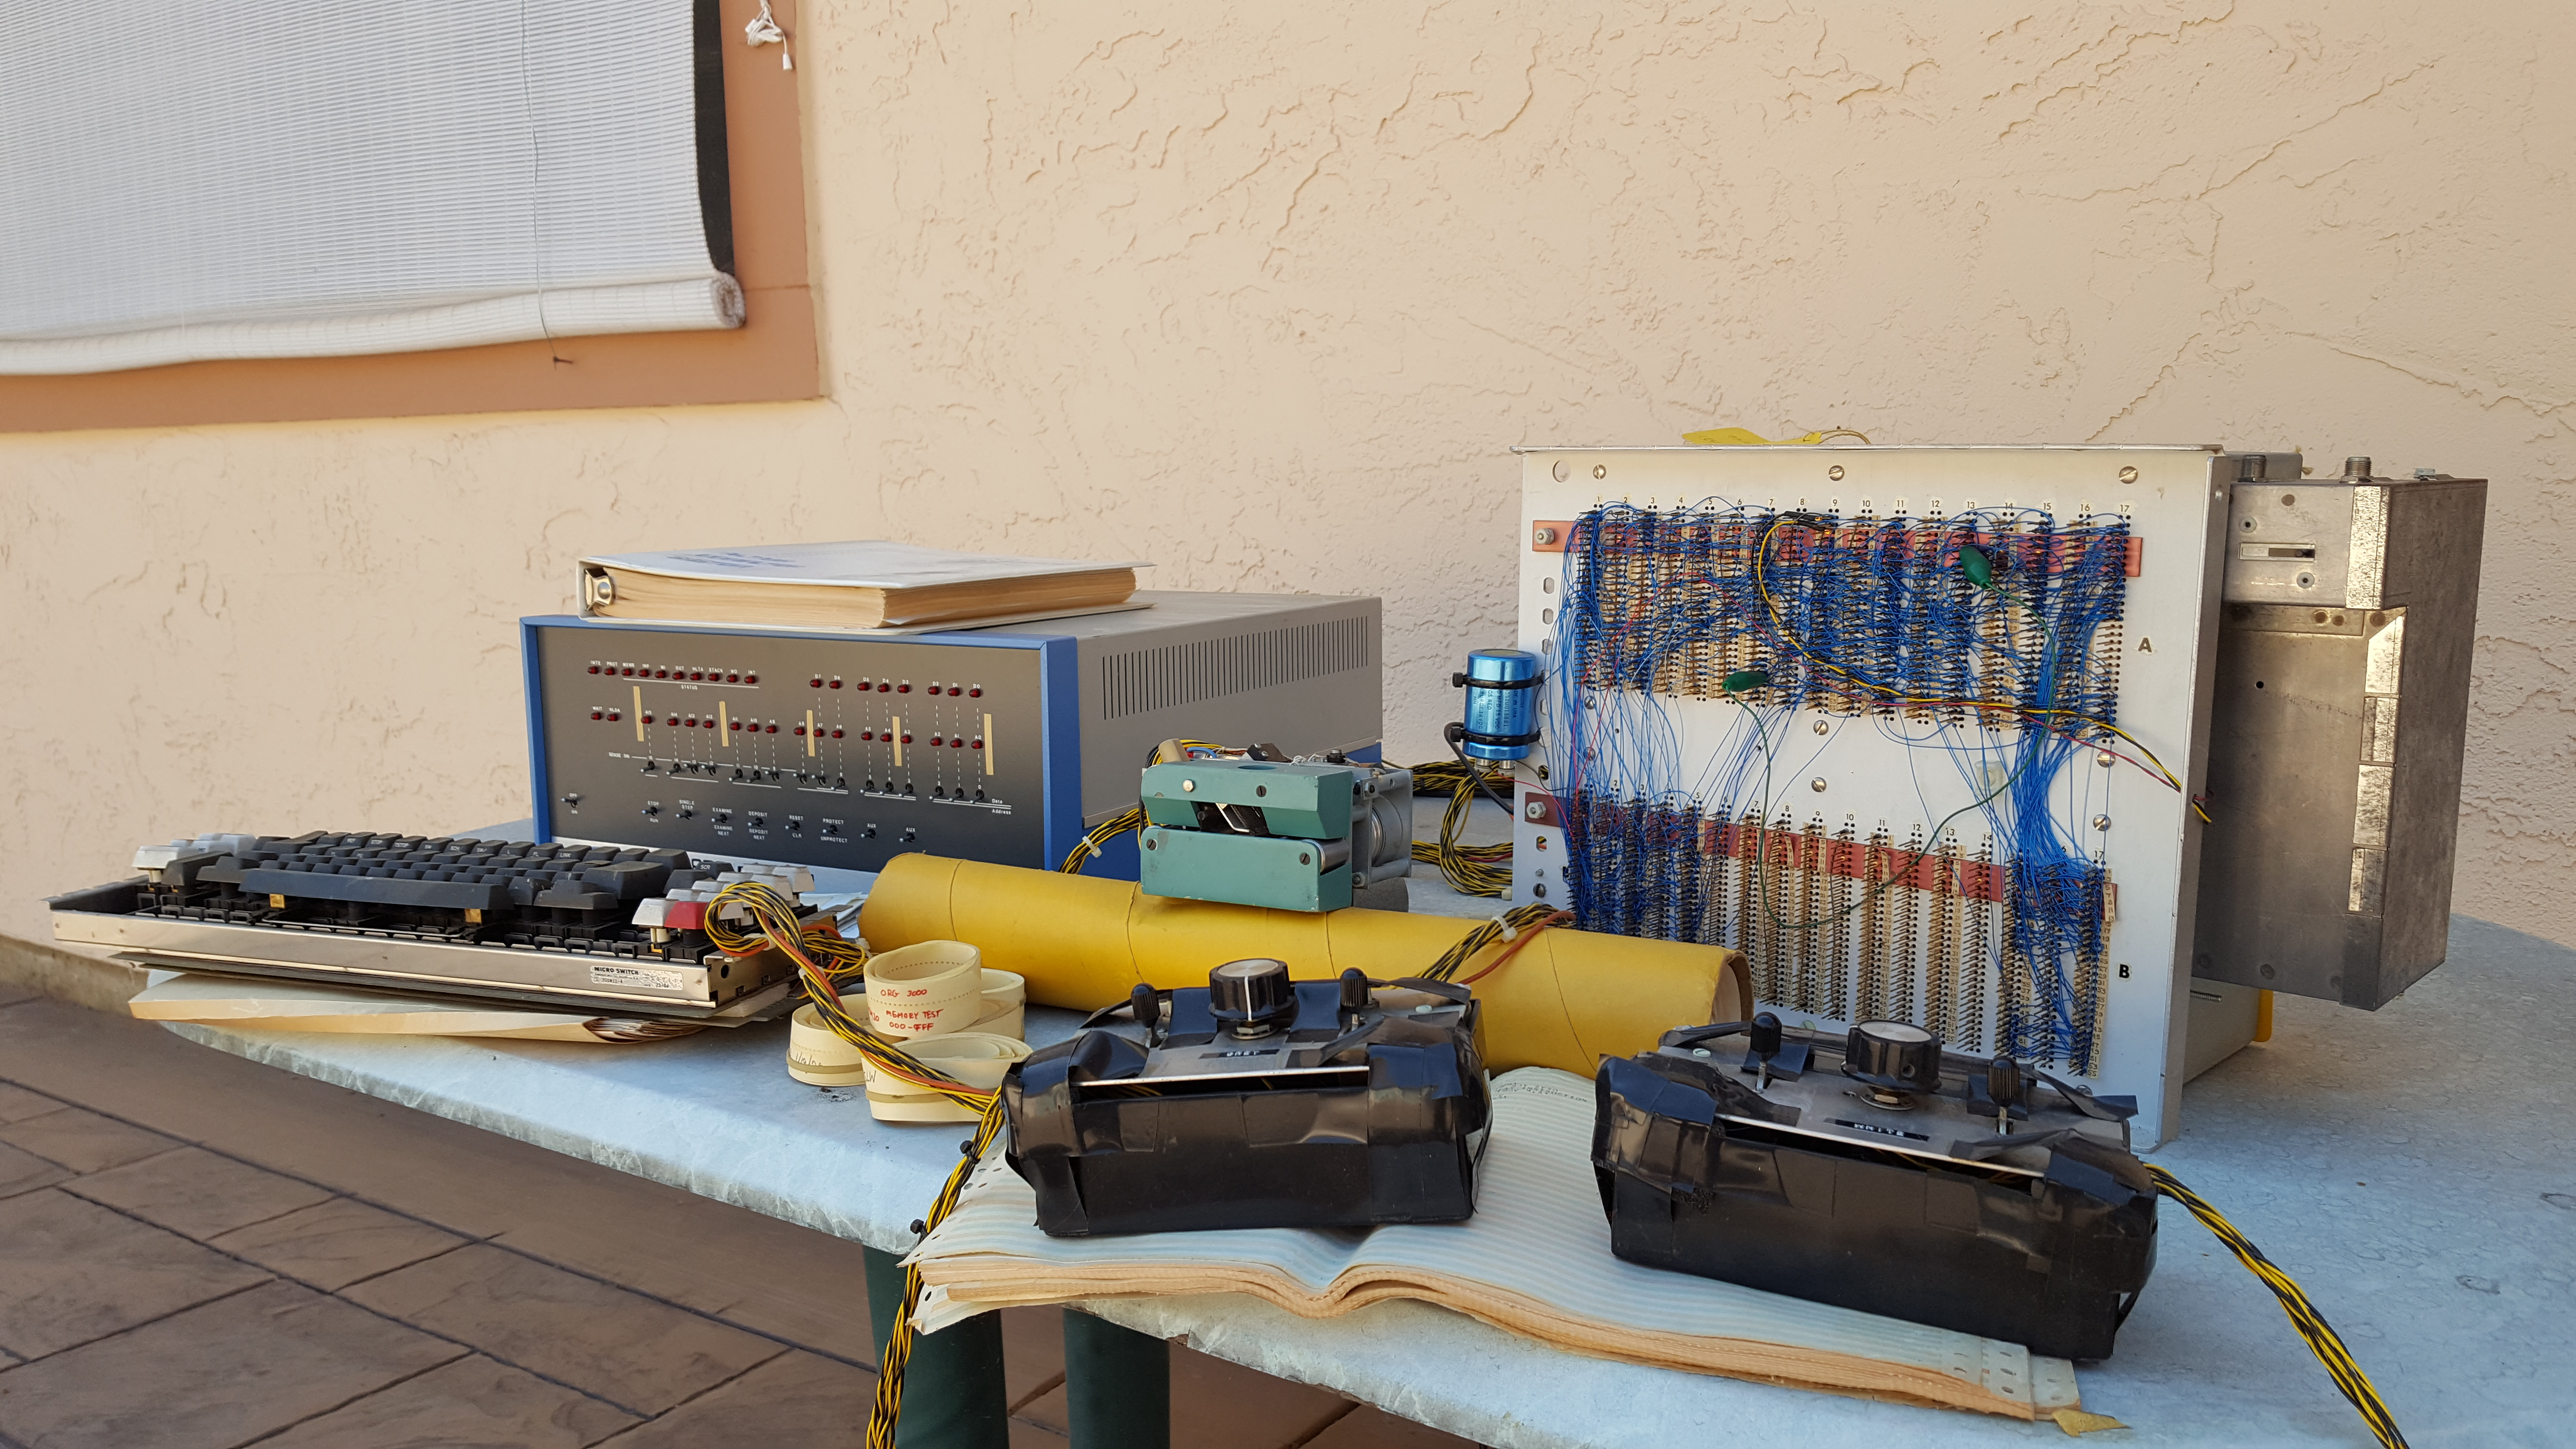
\includegraphics[width=\textwidth]{Pictures/05-ShepperdAltair01.jpg}
    Side Note: David Shepperd kept this Altair system from over the years and provided some photos of it for this work. The machine is now held at the Strong Museum of Play in Rochester, New York.
\end{tcolorbox}

All the logic I dealt with at DeVry and all times later was simple TTL. I thought it was great (still do). When it came time to do a video system, I didn't know exactly how to put a picture on the screen, so no I had no guide in this regard. All I knew was what was necessary to produce an H and V sync signal and that by varying the input voltage between the sync pulses the TV would show either a bright or dark dot. It seemed like it ought to be easy enough. The H and V were digital, so it ought to be real easy to put a digital signal between the sync pulses too to make the TV show something.

The resolution of the screen is what threw me off. Broadcast TV had two frames of 262.5 horizontal lines for a total of 525, but that's not divisible by 512. So what to do? How many binary dots can I put on each line? Is 256 too few? Is 512 too many? 

512 of anything at the time meant another memory chip or another counter (counters were 4 bits each, memory chips typically were 256 bits each). Overflowing into an extra counter or memory chip made things more complicated and took up more room on my tiny circuit board. I decided to start big and made my sync chain do the right thing and make two frames of 262.5 lines and draw 512 pixels per line. 

My idea was to make the thing as general purpose as possible, but it didn't really work very well. I wanted to have lots of sprites I could move around; I think I settled on just two but I could duplicate them. I had two 512 bit memories for each sprite, one for horizontal and one for vertical. I could set a bit in the horizontal (H) memory to start the sprite display. It would display at each point on the horizontal where a bit was set. 

I don't think the bit auto-reset, I think the CPU had to clear it during vertical blanking. Likewise for the vertical. For each vertical bit set in the memory, the sprite would start a display (it had to have both a horizontal and vertical (V) bit to display). Imagine tic-tac-toe lines on the screen with a line wherever a bit is set in either the H or V memory. Wherever there is an intersection, it would draw a sprite (the same sprite).

I believe the sprites were 8x8x2 pixels. The two bits provided some greyscale (off and 3 levels of grey). I believe I chose that because Pong was out by that time and I wanted to make sure I could do paddle games with arbitrarily-sized paddles which I could do by stacking sprites vertically. I never made a paddle game with this hardware though. 

\begin{tcolorbox}[]
        {\InsertBoxR{0}{ 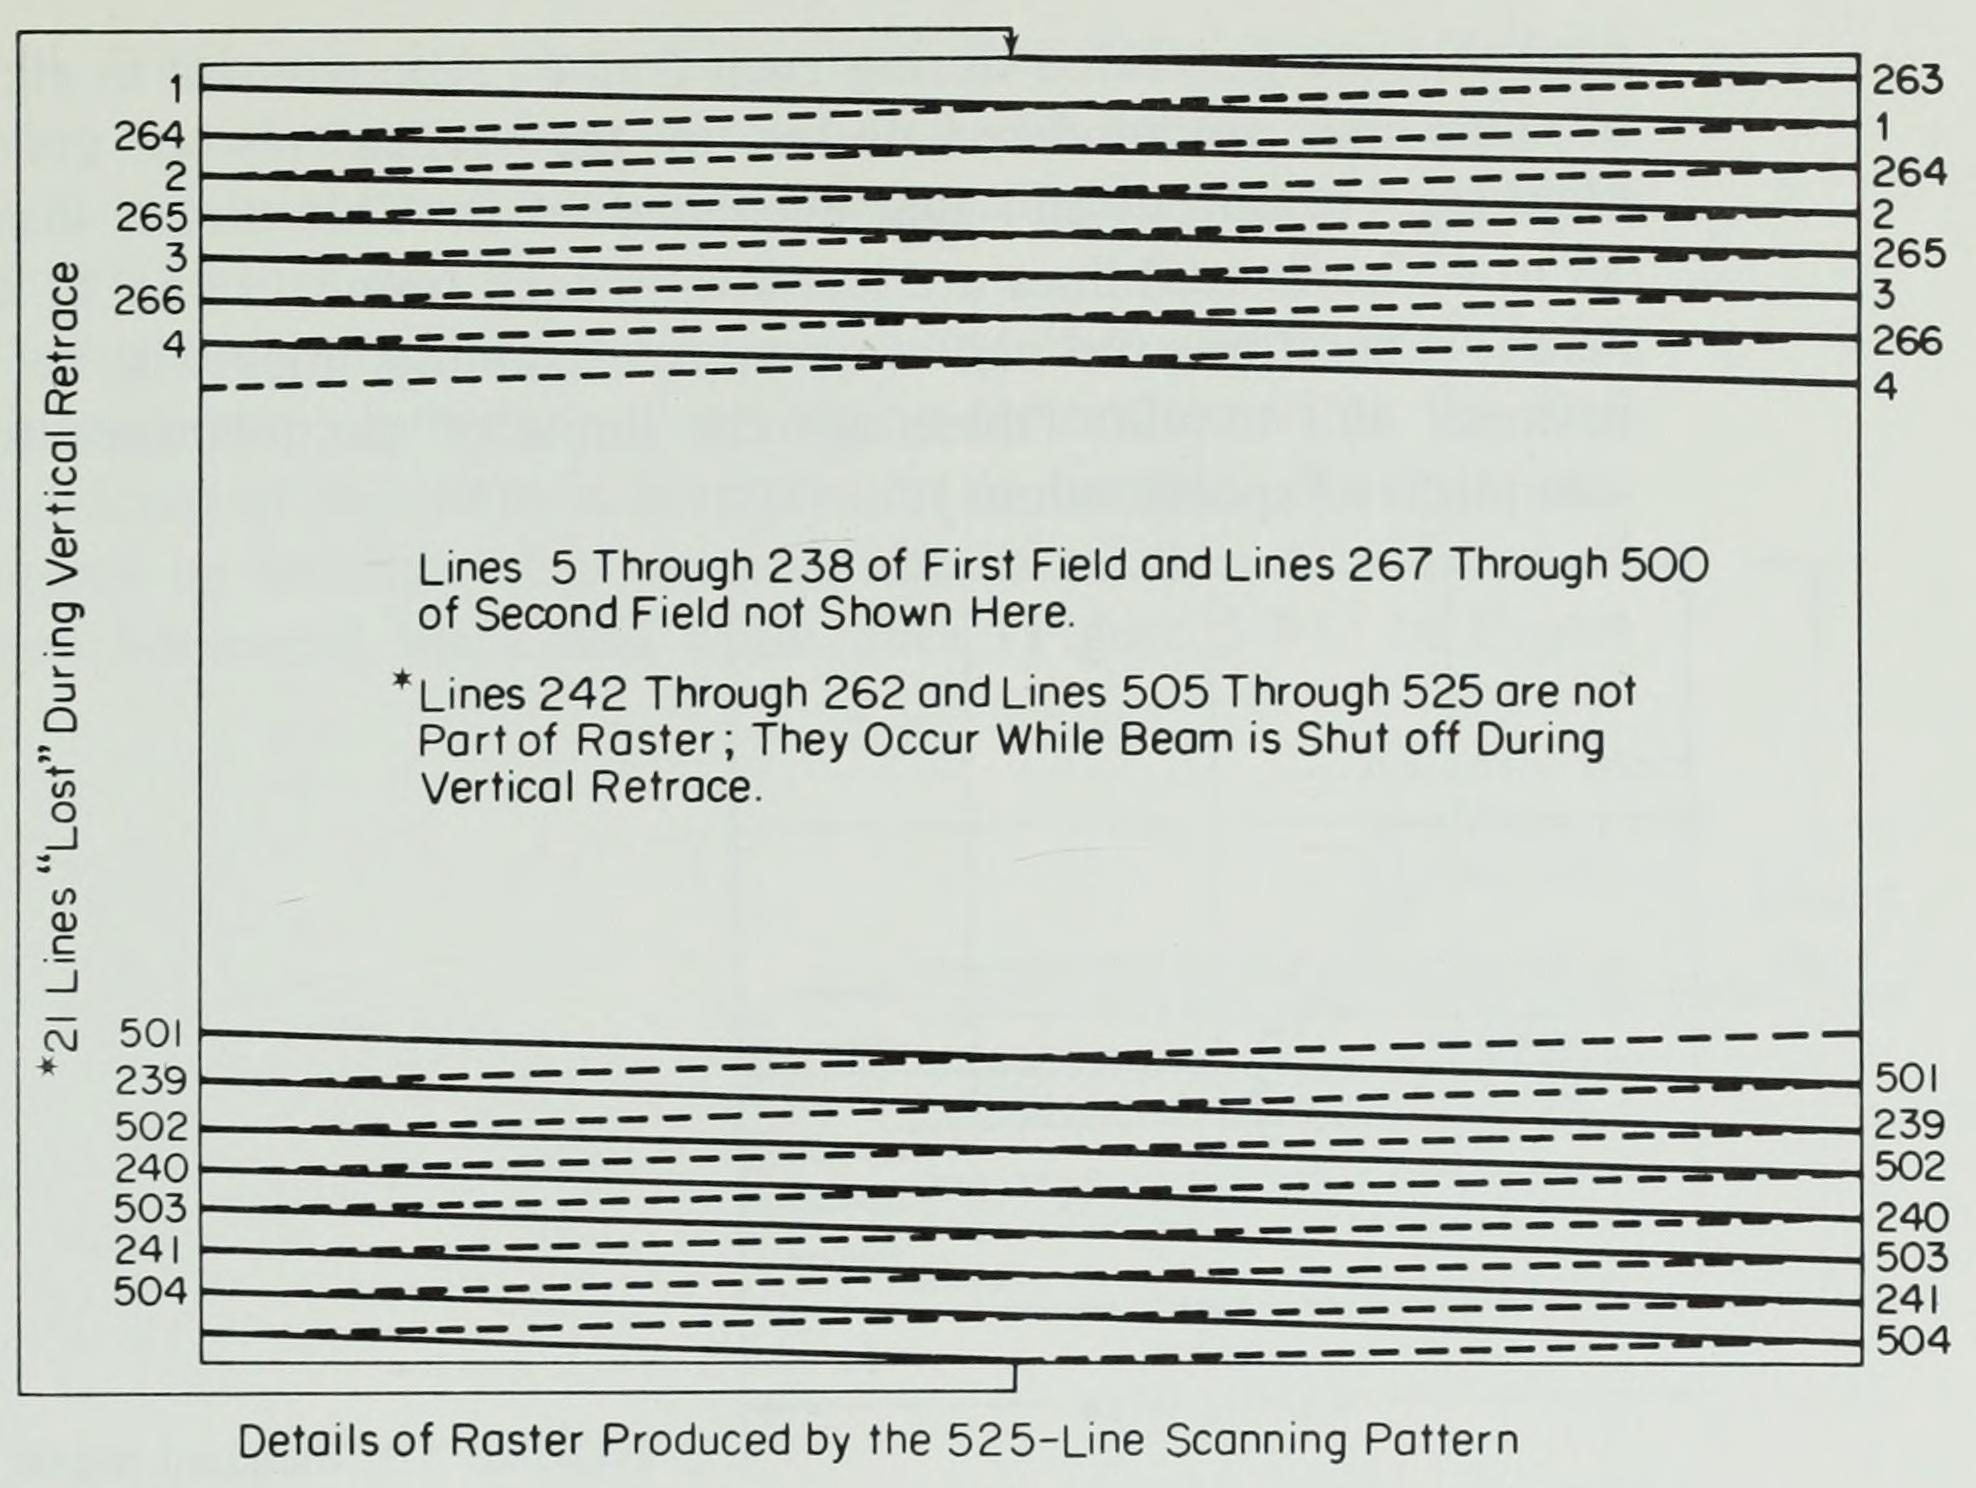
\includegraphics[width=.5\textwidth]{Main Folder/Pictures/05-RasterScan01.png}}
        Side Note: The problem Mr. Shepperd describes refers specifically to the method that a picture would be displayed on a tube-style television. The issue with the line count (horizontal strips that make up the television display) is that data is stored in powers of 2, like 512. To fill a 525 line screen he would have to include an extra chip, which would create a lot of expense for additional, unused memory. Pioneers in the field like Ted Dabney at Atari solved this issue in various different ways, but Shepperd was among the first to attempt a full bit-mapped system as seen on computers today.\\ Figure from "Introduction to Solid-State Television Systems, Color and Black \& White" by Gerald L. Hansen}
\end{tcolorbox} 

The playfield (as we called all background images) I made for this hardware, I believe was just a giant array of bits: one bit per pixel. I don't think it was 512x512x1. It might have been a 256x256x1 and I drew each bit twice in a row (this is probably what I did). 256X256x1 is 65K bits of memory and that was hard to come by in 1975. 512x512x1 would have been out of the question, although I remember using lots of crap DRAM I was able to get from the scrap bins at Intel. So, maybe it was 256k bits. 

The only games I made with this hardware didn't change the playfield much. There was a draw function to place things here and there and I might have had a game where a crash would leave a spot (I don't remember). My Altair system did not have an output device so there was no way to save anything. I had a paper tape reader to get stuff loaded, but no printer or paper tape punch. I had to copy any changes to paper then manually enter them later if I wanted to run something again. 

To be clear, with my hardware, the Altair didn't participate in doing any video. All the video was handled by TTL circuits. The 8080 would just set some registers during vertical blanking and go to sleep. I remember measuring the processor time and it seemed to me it took well under a millisecond to execute all of the very simple games I ever made on this hardware.
I didn’t use ROM in my hardware. I stayed away from anything like ROM for the simple reason that it was not changeable. Remember, my design goal for the thing was to be changeable by just loading a new program. So everything was RAM based. The 8x8x2 pixels in the sprite: RAM. The playfield memory: RAM. Program memory: RAM. 
There were no EPROMs available (to me anyway) at the time. Even for the first couple of years at Atari we didn't use EPROMs: too expensive, too unreliable, not big enough (too few bits), etc. Before EPROMs we used bipolar PROMs which were very expensive, use-once gizmos. Atari didn't like RAM. They put as much as they could in ROM (or PROM or later ERPOM) and put as little RAM on the game boards as we could get away with.

As an aside - and also as a treat to myself to be able to use my Altair for something more useful than gaming - the company I was working for at the time had designed a whole new product with dozens of circuit boards each containing dozens of chips all wire wrapped. It was my job to test the wire wrapped boards as well as help test and prove the designs. It occurred to me I could make a test jig accounting for the 100's of inputs and outputs presented by the board under test with open collector drivers, pull-up resistors and normal input buffers. It cost an extra couple of days to make the jig, but nobody complained. 

Then I just had to write a program unique to each type of board under test and have the computer wiggle the appropriate inputs checking that the outputs do the right thing allowing for scope loops and other things to make it easier to find and fix problems. The thought was if at least each of the boards can be proven to do mostly what they were supposed to, then when all of them are plugged into the backplane of the unit, it was more likely to work as a system. I believe it worked as planned.

\textcolor{interviewer}{Interviewer:} So how did all of this turn into a job at Atari?

\textcolor{interviewee}{David Shepperd:} In late 1975 I saw an ad in the local newspaper. Atari was looking for programmers. As it happens - at the same time I was doing it - the guys at Atari had the same thought process about using a microprocessor in their games instead of hard wiring everything, but they had no programmers. They needed some help, so I sent in my resume and they invited me for an interview. 

I packed up my Altair and video system and took it to the interview and said I'd hook it up and show it to them, but they weren't interested (I learned later, they couldn't for legal reasons). At the time of the interview they asked what I wanted to do and I said either hardware or software. They said they had only an opening for software, so right then I decided to change my career path to software. Although technically I was a programmer, at Atari anybody could do anything if they showed both interest and competence, especially in the early days. That was my experience at least, so I had plenty of opportunity over the years to do hardware design, build, test, debug too.

\textcolor{interviewer}{Interviewer:} Why couldn’t they look at your Altair game? Wouldn’t that have been a good example of your prowess?

\textcolor{interviewee}{David Shepperd:} The reason they wouldn't see my work was quite simple: although I called it a legal issue, it wasn't because of some law or other. Atari was afraid I would drag them through the courts should they see anything I did, not hire me, and subsequently ship product with some aspects of it that matched my work, intentionally or unintentionally. This was very common practice then and I believe the same is true today in most if not all industries. It remained true the entire time I was there not to solicit or accept from anybody outside the company any idea for a game. 

During the interview with Tom and someone I can’t remember I guess just trusted what I told them of what I'd made just by asking very pointed technical questions. Stuff like: "How did you manage to hook it up to a television set? How much CPU time was spent doing X?"

I was the second programmer hired at Atari (at least I believe those with a title of programmer; there were a couple of guys working in a branch office in Grass Valley, CA who were hardware designers but also doing a bit of programming). It was as a programmer that our main task was with the programming of actual game code. Tom Hogg (the first programmer and my boss at the time) and I also had as our charge the care and feeding of the two DEC mini-computers used first by us and then all the subsequently hired game programmers.

When I started with Atari they were just coming off a wildly successful coin-op product, a two player tank game: Tank, but had been struggling for the 3 or so years before that. I believe it was this influx of cash and goodness that enabled them to begin a hiring frenzy of game programmers. I'd been told prior to this time the employees' paychecks would bounce on occasion and/or be told when given their paychecks "Don't cash these for a few days" and stuff like that. 

The coin-op labs had been equipped with second and third hand test equipment. The cast was set such that whatever it was we made, it had to be cheap to build. I seem to recall the magic number at the time for the cost of building a game was not to exceed \$1000 parts and labor (this is coin-op product of course). We nickel and dimed every bit of hardware: electronics, cabinetry, controls, artwork, etc. 

\textcolor{interviewer}{Interviewer:} What sort of tools were you using to create games in the mid 70s?

\textcolor{interviewee}{David Shepperd:} When I started, there was one PDP-11/05 in use. Tom was the only programmer so it was his and because he was the only programmer it was the only development system needed. Before I showed up, however, they had ordered another, second or third hand, PDP 11/20 which had showed up in pieces a couple of days before I did. 

My very first job was to figure out how to get that PDP 11/20 put together and running. It would be my machine, at least at first. I had never seen a PDP 11 before. Both of these systems had dual 8" floppy disk drives and a paper tape reader/punch. I don't remember exactly the memory in each, but for some reason I'm thinking the 11/05 had 20K and the 11/20 had 24K. The 11/20 had core memory. The 11/05 had semiconductor memory. Both ran DEC's single user RT11 O/S booted from floppy disk (it might have been RT11 version 2.0). 

We used those PDP11 computers from 1976 until 1981 when they were replaced by our first of many VAX 11/780 systems. The PDP11's continued to run single user RT11 the entire time we had them although at some point in the late 70's we were able to put Winchester hard drives on them so they didn't have to boot from floppy anymore. I believe the consumer division had a PDP11/34 and they were running either TSX or RSX (maybe both on different machines?) I know RSX was DEC's O/S and I think TSX was a product from someone other than DEC but both were timesharing O/S.

In the earliest days, our programming paradigm was what would be called at the time "batch processing". You may not be familiar with the process, but back in the olden days (I never think of them as "good 'ol") of mainframes before time-sharing, mini-computers, and terminals, there were card punches. Programmers would write their programs on paper, sit at a card punch and transcribe their program into 80 column Hollerith cards (or have a clerk do it for them). Hand the stack of cards to a computer operator. Wait some time for results. Come back (much?) later to collect their results. Rinse and repeat. 

In our case, the results of our code were in the form of a printed 132 column program listing and, if there were no assembly errors (everything was in assembly language back then) a paper tape with the executable code on it. The programmer would take that paper tape and get it loaded into their test board by various means. In the very early days, it was via an ASR-33 teletype where - in my experience - one of three things would happen: Either it would successfully read the tape (yeah!); it would misread the tape and I would have to start over; or it would tear the tape to bits. In all those cases it was at the mind numbing speed of 10 characters per second.

\textcolor{interviewer}{Interviewer:} How was the hardware for each game determined?

\textcolor{interviewee}{David Shepperd:} We explored using processors from National Semiconductor (the 2650), Motorola (the 6800) and MOS Technology (the 6502). When I started Tom had two games in active development, one had the 2650 (Quiz Show) and one had the 6800 (Tank 8). The Flyball project had a 6502 in it and I believe most, if not all, the subsequent games developed in 1976 used the 6502. All the games I did until the 1990's used a 6502 processor. We played around with a number of 8 bit variants of those processors too: 65C02, 6809 and others I don't remember. 

\textcolor{interviewer}{Interviewer:} I find it interesting that Atari used the 6502 so much when barely any other arcade company did. I've heard complaints about it being relatively slow with real-time displays, but was that your experience with it? Did it make it easier to develop for down the line because Atari invested so heavily in MOS on the consumer end? I know that the Atari System I and II used 6502s for sound.

\textcolor{interviewee}{David Shepperd:} I think you have to keep in mind for our coin-op product, the displays were always performed in hardware. We in coin-op were much more free to throw additional hardware at at problem than was consumer, for example. In most of our games, the micro-processor was mainly a steward for the display, did the game logic, handled control inputs, audio and coins. 

Yes, it was sometimes too slow to do all that but in those instances we found cheats and other workarounds. The 6502 in the consumer product had a lot more work to do and basically had to do all the game logic during the 1.5 milliseconds of vertical blanking. Apple chose the 6502 for their Apple II product but I do not know why it wasn't used by more widely. I liked that processor and found it very easy to code for.

As for creating games, this was a wide open area in the earliest days. When I started the hardware for my game, Flyball, it had already been designed and mostly tested by Richard Patak. However, there was no gameplay designed for this original platform. As far as I know, nothing other than a broad idea of "Let's make a baseball game of some sort". As it happens, neither Rich nor I knew anything about baseball. 

For me, just what I remembered from grade school recess, not that it would have mattered in this case since the hardware had only one sprite which displayed the baseball (a small square). Anything else that need to be displayed had to be done in what is called the static playfield (imagine playing a game using just ASCII graphics on a 80 column by 24 line terminal; it wasn't as coarse as that, but similar in concept).

\textcolor{interviewer}{Interviewer:} The former marketing manager of Atari coin-op, Frank Ballouz, mentioned that he had Flyball recalled because you could walk the player on third base to home. Do you recall that issue and any other features of the gameplay?

\textcolor{interviewee}{David Shepperd:} As mentioned earlier, Rich Patak designed the hardware and I think it was done and mostly tested before I even started at Atari. There was no game-play designed before I sat down in front of it, so I have to take some credit for coming up with whatever game play ended up on screen. It was my first programming of a 6502, the first use of RT11 on a PDP11, the first time in a game design environment, etc. Plenty of firsts there. Probably it is what helps with the memories about it. 

The story about the game, although apocryphal (and heard by me second hand) I can testify the game does have that bug. I cannot say if I knew the baseball rule at the time (possibly and equally possibly not), I can say it never occurred to me that my scheme would not work and could easily be defined as a bug. 

I have a recollection of keeping track of players “on base” using a single byte (bit 0 = player on first, bit 2 = player on second, bit 4 = player on third). On a hit or a walk, I would just do a shift left of that byte. If, as a result, any of the odd bits were set (bits 1, 3, or 5), the corresponding animation would take place advancing the player to the next base. When the animation was complete, one more shift left (rotate actually, with possibly rotating in a bit to bit 0 for the player reaching first base). 

If bit 6 was set as a result of this last shift, a player reached home and count it as a score. Simple enough and works okay for hits and runs, but fails badly for a walk if there is an empty base between base runners. A single byte used (I don't remember how much RAM that hardware had, but I'm thinking it could have been as little as 32 bytes for variables and stack; it might have been 64 bytes.) The story I heard is the location (a bar?) where one of these things happened was torn up by the two players who got into a huge fight because of it.

How did I come up with the game play for Flyball? Beats me. The options were limited. There was one “motion object” (the sprite) that could be moved anywhere. It was just a tiny square on the screen and represented the ball. The pitcher was supposed to pitch, the batter was supposed to hit, then what? I just figured the pitcher should use his joystick control to run after ball once hit, pick it up then try to tag the still running player before he got to base. The batter could control the hit by how fast and when he swung at the ball. The boss wanted the pitcher to be able to steer the ball on the way to home plate, an idea which everybody in engineering thought sucked, but the boss gets what the boss wants.

\textcolor{interviewer}{Interviewer:} Before Flyball you did Night Driver, right? You’ve mentioned in the past that Night Driver was based on viewing a flyer for a German game. What do you recall about the creation of it?

\textcolor{interviewee} {David Shepperd:} As I have said before about Night Driver, I just don't remember very much about what was on that flyer I was allowed to look at for a few minutes. Oddly, I remember the circumstances about the receipt of the flyer more than what was on it. My memory about that could be bad too, however. 

I seem to recall it being warm in a crowded office. But all the offices were always crowded on the Division Street building there in Los Gatos. I was probably sitting at a (my?) desk perhaps contemplating my next project or finishing up on Flyball when somebody (Lyle Rains?) dropped in and handed me the flyer. I don't remember what was said about it at the time exactly, but I think it might have been something like “Take a look at this and tell me what you think”. I recall thinking or saying I needed more time to study it (maybe I was very busy with something else at the time?) but was told, “Nope”, I couldn't keep the flyer and had to hand it back right away. 

How long was “right away”? I don't remember that. I know for certain I couldn't keep it over night, but maybe they let me keep it for a couple of hours until I finished doing whatever it was I was doing? 

Then when they came back to collect it, I had to quickly scan and commit to memory the only parts of I thought important. Whether it was a single sided Xerox copy of the one side of an actual flyer or a genuine glossy I couldn't say (I'm thinking Xerox copy). I have only a memory of the flyer showing a few reflectors, maybe 3 or 4. Also, I have a vague recollection of the cabinet being turned more at an angle. And the language on the flyer was definitely not English. It could have been German. 

It is very likely marketing had gotten wind of the 3 other projects like this currently in development by other companies and about to hit the market and was hoping we could beat them to the punch. So I think the project was a “hurry up and do this” so we can get out first, but since this was only my second project at Atari, I don't remember feeling that pressure as being out of the ordinary.

\begin{tcolorbox}[]

        {\InsertBoxR{0}{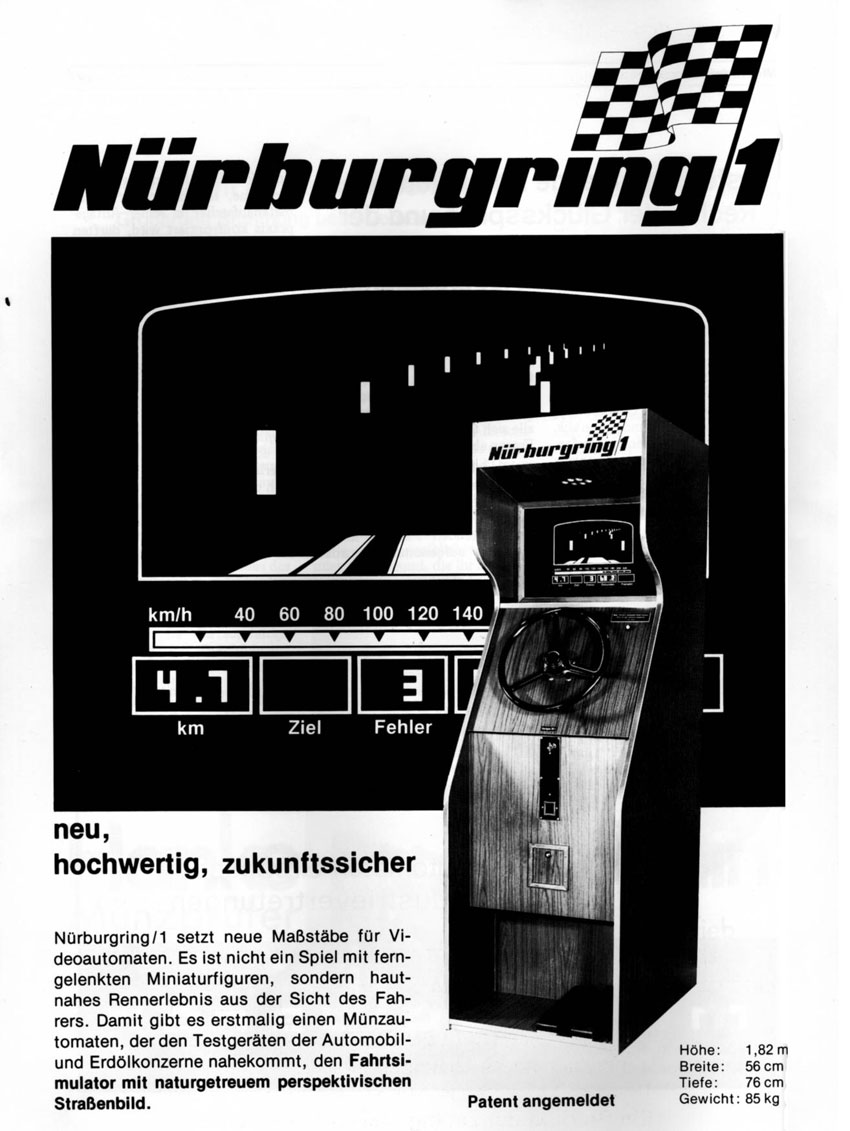
\includegraphics[width=.5\textwidth]{Main Folder/Pictures/05-NurburgringFlyer01.jpg}}
        Side Note: The German racing game being referred to here is the 1976 arcade game Nürburgring, released only in Germany. That game would be massively influential as three clones of it appeared in the US that year alone. By happenstance, Shepperd’s Night Driver would be the first released.}

\end{tcolorbox} 

A few other vivid memories of the Night Driver development. The hardware was based on a very clever design by the engineers at Grass Valley. They called it MOC16 for (Motion Object Control [times] 16). It allowed for 16 sprites to be placed anywhere on the screen. I believe in their design, the sprites could be 16x16 and it might have first been used on the tank 8 game (8 tanks and 8 shells, one each). Terry Fowler took that design and modified it for Night Driver stripping out a bunch of extra stuff. Our sprites were all just rectangles of differing sizes so were pretty easy to draw in hardware.

Before I had written one line of code, I remember driving to and from work along the freeway watching the behavior of the fence posts, lamps, signs, etc. whiz by trying to imagine how I could make those little rectangles appear to do the same on a TV screen. If you are thinking of 3D math, and matrix multiplication on an 8-bit 1MHZ 6502... Sorry to disappoint. Nothing as exotic as any of that. 

I did use 16 bit arithmetic for some of the values maintained for each 16 objects. However, I learned once it was complete, I could have used 8 bits for those and it would have worked fine and probably have been plenty precise enough. But the processor was not pressed for time or memory so it didn't much matter. Some of the variables for each object were kept as 16 bit fixed binary point fractions with the binary point between bits 14 and 13 (15=sign bit, 14=2\^0, 13=2\^-1, 12=3\^-2, etc.)

I remember having cooked up and coded up this whole scheme with the math, figuring out how the rectangles might move both top to bottom and left to right, choosing their size, etc. and haven gotten my paper tape and listing with all this stuff in it never been run before. I coded it such that all the things I wasn't sure about could easily be adjusted on the fly with just a patch to a variable. I sat down in front of my hardware with paper tape in hand preparing to put it in the teletype when the project leader came in to see how the project was going. 

I said to him, “I'm just about to find out for myself for the very first time whether any of this is going to work and what this is going to look like”. We waited while the tape loaded. I told the AtariJolt to go and Night Driver was born. It all just worked right out of the box. The rectangles spread top to bottom and left to right just as I had hoped. With the project leader sitting there, we made adjustments for the position of the horizon and I changed some of the characteristics of how much the top-to-bottom and left-to-right spread there was.

One other notable thing about this game. It was extremely popular among the company personnel. There was a more or less steady stream of people from all over the company constantly coming through my lab to see the game in action. It was more than a distraction to me since it cost me precious development time while they were doing their dog and pony show and/or wanted demonstrations of the work in progress.

\textcolor{interviewer}{Interviewer:} Would that include executive and marketing personnel like Gene Lipkin, Nolan Bushnell, or Don Osbourne?

\textcolor{interviewee}{David Shepperd:} I don't remember marketing being much of a bother on any of my projects (though I could easily be mis-remembering). But Lipkin, that's another story. I believe everyone in engineering cringed when word came down that Gene was on his way to look at the stuff in development. Many times Gene wanted changes that completely upended the current development or even he'd be unhappy with a project still in early stages of development and quite apt to cancel it. 

If an actual project review was not scheduled for a particular game, the game team would throw the “Lipkin switch” on the hardware (basically it just turned off the monitor) so if Gene walked by he wouldn't even notice the game or if he were to ask, the team would just say “sorry, the hardware is broken right now”. I only saw Nolan once in a great while after I started. He too would walk through the labs checking out games in development, but by the time I started Warner Communications had already started making plans to give him the royal boot so I think he had other fish to fry. I was not privy to any of the goings on in either middle or upper management. 

\textcolor{interviewer}{Interviewer:} In addition to the “Lipkin switch” you mentioned earlier there was also an Atari tradition called the Stubben Test.

\textcolor{interviewee}{\textcolor{interviewee}{David Shepperd:}} Yes, the Stubben Test was run to see if the cabinet and/or controls could be broken, but there was also the all important Owen (Rubin) test. Owen had an unbelievable knack of breaking everybody's "iron clad, unbreakable" game code almost right away just by finding just the right combination of control inputs to tickle those odd cusp conditions in the game code not accounted for and blow the game up, cause a crash and reset or cause some very odd unpredictable game play. I don't think he did it on purpose either. It was just his normal way of playing that managed to find edge cases. You should get Owen's take on things. His stories won't disappoint. 

\textcolor{interviewer}{Interviewer:} Who were the people you had the most contact with in the coin-op division? I've always heard great things about the camaraderie between the engineers, so how did everybody play off each other? 

\textcolor{interviewee}{David Shepperd:} I don't remember the names of all the people I worked with over the years. Who was more influential than others? I am sure that changed from time to time. The first of us programmers, Tom Hogg, Ed Logg, Mike Albaugh, Owen Rubin, Dennis Koble were among them. Lyle Rains was a big influence and I worked with him directly many times. 

I'd put Lyle up there in the genius category. He was an excellent artist, game designer, hardware engineer and he was a programmer too. He wrote a number of development tools for us. I don't think he cared much for the management duties he got drafted into over the years. At one point he became a "Fellow" which I think allowed him to do whatever he wanted without schedules, meetings, reports, etc. He had no nobody reporting to him but I don't believe he had any trouble getting people to do little things for his pet projects, after hours and under the table, of course. That would include me.

He and I did the animations for the 20 year anniversary movie for Atari. I believe he did all of that on his personal Amiga he brought in to work from home. I think he wrote the program that would do the frame rendering and I must have been the one to port it to run on all the Unix like machines we had in the company at the time (I think we were running SCO Unix, Esix, SunOS and maybe one other on various PC's equipped with 386 processors (there were three Sparc II Sun systems). I'm not sure I had the VAXen do any of that rendering work or not, probably not. 

They were all networked together with Ethernet and I worked out a Perl script that would basically do what Boinc does now: gather finished renders and ship a frame needing rendering to the next available machine. Some machines were very slow and took hours to render a single frame. I think the Suns could do one in less than 30 minutes or so. Still there were 1000's of frames to render, I would start the "render farm" running only at night after everybody had gone home and I remember there was a time when we looked at the number of frames left to render, the time it took on average to do them and didn't think we had enough time or machines to finish the job before the deadline. But we made it.


In my line of work there I probably had dealings with nearly everybody in engineering, both hardware and software, very often and with obviously some more than others. I don't know what was going on in the minds of the hardware engineers. I know there was a turnover of hardware designers early on and it is possible they were thinking "There's nothing more for me to do here" or some such and left. But I would have to take issue with that thought process. The needed designs were just different. And the video displays just grew more and more complicated and faster and faster. That frenzy continues to this day mostly between Nvidia and AMD.

What stands out for me in coin-op is the hardware and product (game play) really had to be cutting edge. All the time to be a success. And being hardware based, we could push the envelop with both video systems, controls and cabinets. Think "real" submarine periscopes, X-Y monitors, 25" color raster monitors, dual monitors, mirrors, black lights, trackballs, spinners, force feedback steering, multi-channel audio, etc. The list goes on and on. Of course, most of the more exotic things were only available once we started making more money than we knew how to spend fast enough.

\textcolor{interviewer}{Interviewer:} Which games did you have personal production involvement in? People have collected credits over the years for Atari employees but some may not be accurate.

\textcolor{interviewee}{David Shepperd:} As for games I worked on directly, I can tell you I coded up Flyball, Night Driver, Sky Raider and Asteroids Deluxe. I coded up a few others that never made it out of the lab. I don't remember the names of all of the unreleased games I worked on with the exception of Mini-Golf. Other games I may be credited for may just because the game's producer (or programmer) felt generous and is no doubt something to do with the many of the development tools the game programmer ended up using. I did not contribute anything to the game play or design of those other games. For the later higher end games I was responsible for much of the operating system content that we ended up using in them; no help with the gameplay.

A note about credits appearing on screen. The company frowned on doing that for many years in the early days. I believe management was afraid it would make it much easier for poachers and other head hunters to get the names of the prized developers and Atari would lose out. 

I don't remember what or when it happened where they relented and started allowing the names of the contributors to appear on screen. Sometimes the game team would put everybody's name up there, even those who may have just walked by and played the game once while it was in the lab and made a remark (think of those miles of rolling credits after a movie). There's a chance my name is among them for that reason. Others were more discriminating and only listed those directly involved in the game design and development.

\textcolor{interviewer}{Interviewer:} How long would the production schedule – from programming to production – take for those late 70s games? I’ve heard that games like Breakout were consistently delayed before they got there. What was standard project cycle like?

\textcolor{interviewee}{David Shepperd:} In the early years (1976-1979), I think from concept to out the (engineering) door, it could have been as short as about 6 months. That was just with maybe one or two developers (maybe a game designer and programmer; sometimes the programmer was the game designer too). That time exploded into many more man months as the video systems got more complex. 

Doing the audio and graphics became way too much work for one guy, so soon the projects grew to need several support people (graphics and audio designers were shared among all the projects) and the games themselves became more complex needed more time to work out the details and make it fun. The first games only needed around 4k bytes of memory. 

Measure how much memory is needed by some of the games today. Some of the simpler games I play on my PC need 4GB of memory (disk and main memory) to hold all their code, data, graphics, etc. That's 1 million times as much raw data. One should not be surprised that it takes a team of 50 or more as much as 2 years or more to get that game out the door.

As for my projects specifically, I am not sure. I know my first one, Flyball, was complete by the middle of 1976 and I am pretty certain my second, Night Driver, was also complete by the end of 1976 (we moved buildings at the end of 1976 and I was done with ND by the time we moved). So those two probably were done in less than 6 months each. 

What I worked on in 1977? I am pretty sure I worked on something that never went anywhere. Then I think later in 1977 and maybe part of 1978 I finished Sky Raider (I am not sure about that, but I do remember being at 1265 Borregas when I did Sky Raider and 1265 is where we temporarily moved into after leaving Los Gatos in 1976. I think Asteroids came out in 1979 and we were in our engineering building at 1272 when that was developed. I don't remember exactly, but it must have been 1980 or 1981 when I did Asteroids Deluxe. 

How long did it take me to do Asteroids Deluxe? I can't say, but I don't think it was much longer than 6 months. It might have been 9 months because I was also the hardware engineer on that project. Still, not much in the way of graphics or audio needed with that project and besides Lyle Rains did the graphics and most of the game design for me. We got our first VAX in 1981 so I'm pretty sure I quit the game making about then to become full time tools guy.

\textcolor{interviewer}{Interviewer:} I was looking at the schematics for Flyball and I noticed it doesn’t say how much RAM the game had. I know it was common practice for some game companies to “Black box” components so that competitors couldn’t copy their games, but is that something you would have been aware of?

\textcolor{interviewee}{David Shepperd:} I see from the Flyball manual they purposely left off the part of the schematic that included the CPU, it's ROM and RAM. But I notice from the parts list, there are two 2111 chips unaccounted for in the schematics shown. Those chips are 256x4 SRAMs, so I can infer those two were used for the 6502's page 0 and 1 RAM meaning I had the luxury in the project of having 256 bytes of RAM for both variables and stack. It was a treat I am sure I did not appreciate at the time. 

\textcolor{interviewer}{Interviewer:} How much planning would go into creating one of those early games? Would you have reuse of code for something like the coin receptor or would you rewrite that from scratch every time?

\textcolor{interviewee}{David Shepperd:} I can't speak for other programmers, but I was more of a cowboy about it and continue to be to this day (maybe we all were, except for Ed Logg). Although while in school I learned all about doing flow charts and all those other charts that are supposed to make one's life easier, I never could get behind any of it once I started working (and I still can't). It was always, "I need a function that has X inputs and produces Y outputs", so I'd just sit down and code it directly. 

The code itself was both the flow chart and the comments. In those days it was in assembly and these days it is in C or C++ (but I still code as though I am writing assembly even while writing in C). Sometimes I'd even add comments but rarely in the early days. Comments took too much time to write and they rarely were kept current with the changes. And changes sometimes happened at a furious pace late in the project. I believe comments that describe what the code was doing when first written rather than what the code is doing now, is not at all helpful. Also, in the early days, there wasn't much thought given to code re-use. That changed quickly, however.

One thing to keep in mind is the code in these early projects was actually very small, especially when compared to what we are doing today. In 1976 the project cycle typically was six months from when the game idea was a twinkle in someone's eye to first product out the door and the code writing and debug part of that was probably closer to four or five months. 

I think all the games I programmed for the 6502 fit in less than 8k of pROM. I was never able to get any of my games to fit into 2K. I think both Flyball and Night Driver needed a 4K (byte) pROM. Sky Raider might have also fit into 4K. I think Asteroids Deluxe took at least 8K or maybe even 16K, but much of that was code for the vector generator. 

Figure the 6502 processor needed, on average, 2 bytes per instruction that means the entire game needed somewhere between 2,000 and 4,000 instructions most of the time. I just did a quick line count on the latest microprocessor project I did which took only a couple of months to do and it shows around 10,000 lines of C. 

Maybe you will find this an interesting side note about comments and function and variable names. In the earliest days, our line printers printed on that green and white striped 132 column pin feed line printer paper (in fact, there may have been just one line printer shared between the two PDP11's). The print head was a pinhead with maybe 9 or 15 pins (I forget; it was cheap). The head was dragged from left to right with a stepper motor while pounding those pins through a ribbon to draw on the paper then slap back the left with a load bang. The noise it made was deafening, but I digress. 

What many of us learned early on was we could get our printouts way faster (and quieter) if we packed as little text as possible on each line and the put it tightly to the left edge of the page. That is the printer could print 132 times faster if it only had to print one character in the left column rather than a complete 132 character line, even if some of those characters to the right were spaces (I think all characters took the same time to "print" meaning the head moved at a fixed rate from left to right).

So in the earliest days it would not be unusual to see source code that looks like:

\begin{lstlisting}
        A:.BLKB
        S:LDA I,0
        STA A
        ...
        JMP S
\end{lstlisting}

rather than something more helpful when looking at it a week later:

\begin{lstlisting}
        ACCEL: .BLKB ; ACCELERATION

        START: LDA I,0 ; INITIALIZE ACCELERATION
        STA ACCEL
        ...
        JMP START ; NEW GAME, START OVER
\end{lstlisting}

What we used for debugging the 6502, at first, was this thing called Jolt. I don't remember who made it but it sucked so we copied it and called the copy an AtariJolt. There wasn't much to it, a small pROM and register and a serial connection. We interfaced it to the ASR33 which needed a 20ma current loop and ran at 110 baud. The programmable ROM lived in the 6502's address space that included the reset and interrupt vectors so the code in that pROM always ran first. 

The code in that pROM had a UART [a type of serial connector] emulation to read/write to the teletype as well as provided a simple “monitor” that could be used by the programmer to patch and view memory, etc. I may have written the code that lived in the AtariJolt pROM, or maybe it was written by Mike Albaugh. There was an equivalent thing for the 6800 (Micbug?) but I don't remember if there was a need to make a clone of that.

I remember buying (or somehow getting a hold of) a stepper motor driven paper tape reader. Maybe somebody procured one from somewhere and asked me to get it working with the AtariJolt? It must have needed a special interface. It might have been serial or it might have just had a “go” signal to turn the motor on and off and returned the raw sprocket and 6 hole information which was optically read (probably simple parallel is how it worked; I'm sure it was cheap whatever it was). 

I'm not sure it was I that got it working, but it would have been in my wheelhouse to do that kind of thing at the time. I think once it was proven to work, the company bought a bunch of them and the cabinet people made a little black box to hold it and its power supply. It was way faster and much more reliable than the paper tape reader in that ASR33. For a long time the AtariJolt and that little paper tape reader was our development system for the 6502 projects. 

As I remember it, I'd just code up something I thought might work with the subject hardware then try it out. Either it worked or it didn't. If it didn't I'd work with the engineer and we'd figure out whether the problem was hardware or software or some combination of both. Soon enough we'd get all those details ironed out and I could get on with putting some game play on the screen.

Almost always, the first draft of the game play put on screen wasn't fun. The idea that sounded so good on paper and kicked around in meetings, when put on screen with the controls just didn't pan out. The programmer and game designer (if separate people) would hash out different ideas and try different things. Sometimes the game just wasn't good enough and we wouldn't find that out until the factory was cranking them out by the dozens. 

Other times, the game was so good, the programmer had a hard time getting debug time on the one machine in the lab he had to work on because all the other people in the company would “drop by” to play this new game in development. But oddly enough, even if everybody in the company loved a game and couldn't wait to play it, it wasn't a sure thing the game would be an equally huge hit with players in the field.

As for code re-use. This didn't happen right away. For the first few games, I believe we all rolled our own self test and coin routines, etc. And each of us would re-use our own code from our own previous projects. However, as we learned the cheats the players had used to figure out how to fool the coin acceptors and developed defenses against them, the coin routines became standard and they would get included in everybody's project, but this took a while to flesh out. 

Eventually, the self test functions became standard and they too would get included in everybody's project. Doing so made everybody's job easier since there was much less stuff to write and debug. And if there was a bug fix or new feature to either the coin or self test functions, everybody got it at the same time. I think in the early days, the self test was hurriedly written, mostly as an afterthought, after the game was finished and on its way to production (I'm imagining us thinking, “Why waste time writing a self test for this thing if they are not going to build it?”). 

I could be wrong, but I think for my later projects I wrote the self test first as an aid in the development of the new video hardware and to help the techs (and me) bring up additional prototype boards.

\textcolor{interviewer}{Interviewer:} You briefly mentioned the monitor: How long did it take for your development systems to have their own monitors as opposed to the only output being a teletype?

\textcolor{interviewee}{David Shepperd:} I can't say exactly when we got keyboards and monitors. I do remember the very first ones we got must have been within days (or maybe a couple of weeks) of my starting there, but they were very primitive. The "terminal" was just a qwerty keyboard mounted on a small metal box that had 110vac input, a BNC connector providing composite video out and (I think) a DB25 connector having an RS-232 serial output. 

Since the output was composite video and we had a bunch of monitors we were using for our games, we just hooked up a 12" or 15" game monitor to this box. It worked fine, but Tom had the cabinet department make a pair of cabinets that would each hold a monitor and a shelf under each monitor to hold that box with the keyboard on it. 

The "terminal" displayed just 12 lines of 80 characters and the keyboard provided only upper case ASCII characters and some of the punctuation characters. We may have used them clear up until we got VAXes or they may have been replaced with more sensible terminals at some point (quite possibly DEC VT100's).

Once a third programmer started which must have been a month or so after me, we started up the "batch mode" input I spoke of earlier. We hired two what we called computer operators, Cynthia and Linda. Their job was to type the long hand code we programmers had written on sheets of paper (or the marked up code on a previous listing) into a primitive RT11 text editor, run the assembler and get a listing. If there were no assembly errors, run the linker and produce a paper tape. Package the original input, the assembler and linker listings and the paper tape, if there was one, and put in the "out-basket" for the programmer to pickup later. 

Both Cynthia and Linda got real good at their job and would fix assembler errors on their own and even occasionally "Type what I meant, not what I put down on the paper". The turn around could be quick if there wasn't much in the in-basket or it could be a couple of hours. I know some of us only required one or two turnarounds in a day. 

If we were mainly debugging, we could go all day doing manual patches of our code making notes of the changes on the listings in red pencil. Sometimes it meant manually patching in whole functions to the debugger but those were probably not typical. Then we could drop our changes in the in-basket on the way home from work and pick up the new stuff in the morning. If we had to add lots of new code or there were too many changes made, we would submit for a new tape whenever that was needed.

What I found when I started working at Atari was the lack of adequate tools one needed to do their jobs. It could have been simple stuff like missing scope probes, broken meters and other test equipment, there being only one test instrument that had to be shared among all the developers, etc. I couldn't do anything about that stuff (other than bitch about it). The software tools were extremely primitive too; that I could do something about. 

As mentioned earlier, we were using PDP11's running RT11. The guys at Grass Valley had coded up some macros that could be used with the RT11's macro assembler (called MACRO, normally used to produce PDP11 code) to have it generate 6502 binary (there was a separate set of macros for the 6800). MACRO, being native to the PDP11 family which referenced everything in octal numbers, only allowed for binary, octal and decimal inputs for numbers and produced listings with all numbers shown in octal. With all the microprocessor families we were interested in using though, we wanted to use hexadecimal inputs and have listings show results in hexadecimal. 

There was no way input hex in MACRO so for that we were out of luck and had to use only what it liked (with the resulting requisite occasional confusion and errors). To make the listings show in hex, those same guys at Grass Valley wrote an RT11 line printer driver that parsed the assembler listings on the way through the driver to the printer and converted what it guessed were octal numbers into hex. That driver kinda sorta worked and mostly got it right, but still made lots of mistakes. I used it and groused about it, but none of it was good enough for me. 

You might ask, “Good grief, why didn't we just output the listing to a file, then run a separate program to fix the listing file?” To which I answer, simple: there wasn't enough room either in memory nor on the floppy disks to hold the O/S, the source files and the listing files let alone a second copy of a modified listing file. Nope, the assembler had to output direct to the printer or you got no listing. 

Coupled with that, at first, all programs were best written as a single source file targeted at a fixed absolute memory address. It was possible to write relocatable code and have global variables, but the linker produced a link map with octal numbers which made it clumsy to figure out where the functions and variables were in memory during debugging. One could put code in separate files and fix each of them at different fixed addresses, but that meant the programmer was responsible for manually linking the separate images together to make sure they did not overlap, etc. For me, it was a painful step in code management I thought should be performed completely by the computer.

I put up with it for the first two projects I did at Atari, Flyball and Night Driver, but I was determined to fix that before starting my next project. I believe it was late 1976 when I started coding up a new linker which I called linkm. This tool was going to link all the object files produced by the assembler, produce listings in hexadecimal, allow for dynamic placement of page 0 variables and sections (a 6502 specific thing) and produce a cross reference of global variables and functions. It was written in PDP11 assembly (everything on the PDP11's was done in assembly). I don't remember how long it took to finish and I was probably working on it while I was coding my next game (I don't remember what that was, no doubt one of the many that didn't make it to production). When I did finish it, however, it became the tool of choice for all developers.

I wrote tools that would manipulate input files of various formats to break them into the appropriate pieces needed to program into separate PROMS and ROMS (I don't remember all the different types of PROM programmers we had or how we interfaced to them; some early ones could have been via paper tape). This tool became the standard used for many years. Again, I mainly wrote the tools I needed to help me with my projects as I saw fit and they were quickly adapted for use by all the developers.

At some point after linkm was done, I don't know exactly when I started or finished it, I wrote a new macro assembler family, also in PDP11 assembly, that would accept hexadecimal inputs and produce listing in hexadecimal directly. It was a single assembler, but could be built with different defaults and opcode tables for the various processors we were using or thinking of using at the time. I'm not sure of all the CPU's supported, but certainly the 6502 and 6800. It possibly included the 65C02, and 6809. I named them kind of after their CPU: MAC65, MAC68, MAC69, etc. 

One key thing with the 6800 family is they are big-endian processors [the way they store bits], where most of the others were little endian, as was all the stuff that ran on the PDP11, so the assembler and linker had to deal with them differently. Something the native RT11 assembler and linker were not equipped to do. Linkm could deal with it easily. These tool chains connected me to all the game programmers all the time. They would come to me for support and/or to ask for new features, etc.

\textcolor{interviewer}{Interviewer:} How much did hardware influence game design as opposed to game design demanding hardware?

\textcolor{interviewee}{David Shepperd:} I think that depended a lot on the technology put forward by the hardware engineer. If the engineer was well versed with what the CPU could do, s/he would give more work for it to do. If the engineer was more versed on what the hardware could do, they'd do more in hardware. For me, in the case of Sky Raider, I had the hardware do most of the work. I'm sure the CPU could have done more, but even now, I'm not sure what I would have had it do different.

For Night Driver, there wasn't much choice. Nobody had much experience with microprocessors at the time. The basic hardware was designed by the folks at Cyan. In the case of Night Driver, consumer successfully ported the game (adding extra stuff even) to the VCS and the CPU does most of the work in that hardware. These days, I guess I'd be very tempted to use real 3D matrix transformations since the CPU instructions will execute 1000's of times faster, would be 10's or even 100's of thousands of times faster doing the math and the math could be in floating point and I'd be programming in C or C++ instead of assembly. Back then though, the name of the game was "just make it look like it's doing the right thing". Sometimes that meant using lookup tables instead of computing math (I think all our sin/cos/tan/arctan calculations were always done via lookup tables; it cost memory but it was blindingly fast). The cheats I worked out meant the computations in Night Driver were very simple and fast.

About the time we did Sky Raider, Atari had been cranking out games and making more money than they knew what to do with. So there was some freedom to explore different, as in off the wall, ideas for games and video systems. Lyle Rains had this idea to display a background that hadn't been tried before where each line was comprised of a series of stripes of variable lengths each of a different shade of grey. 

It was a display of serial data. I.e. 5 pixels of grey level 4 followed by 12 pixels of grey level 9, followed by 3 pixels of grey level 2, etc. I don't remember the specifics, but I think it might have been there could be 16 different stripes on each line and each stripe could be one of 16 shades of grey. That would translate to 8 bytes per line and 128 lines (or it might have been just 64 lines) for a total of 1024 or 512 bytes of ROM per playfield. Thought to be a big win for cost reduced hardware yet still have a very exciting and busy playefield.

The display could be scrolled vertically meaning the starting address of the playfield could be chosen by the processor to be any random number. I don't remember how much memory was in Sky Raider for this playfied but there was at least two full playfields so probably 2K or 1K of playfield memory. I designed the hardware for this product and Lyle was the project leader, game designer and worked with the graphic artist and did a bunch of the video graphics. This thing was more of a proof of concept, but we put in some targets and made it into a game of sorts anyway. 

I was never happy with the game play. I thought it was pretty lame, but the technology was very interesting and absolutely a blast to work on. Atari at the time could sell a bunch of just about anything, do it sold well enough I guess. Designing a playfield under those constraints, however, was terribly difficult. Lyle and I (mostly Lyle) had to re-work what the artist came up with since it did not conform to the strict requirements of "only 16 different stipes per line". 

I remember the design was delivered on this giant piece of vellum marked with different shades of grease pencil representing each of the shades of grey. Lyle and I labored for a long time transcribing those colored stripes into binary then massaging the numbers to get something to look reasonable on screen. It was torture for all concerned. We never did it again.

\textcolor{interviewer}{Interviewer:} So Sky Raider didn’t have any programming which made the 3D effect possible? Didn’t Richard Patak also work on that game as well as Flyball?

\textcolor{interviewee}{David Shepperd:} For Sky Raider the display was done as a complete cheat. Sorry if this is where you find out how the sausage is made, but there is no computed perspective in that game. Nope. 

As mentioned before, I already knew how TV's worked and figured we could make a simple patch to the vertical amplifier input directly in the monitor to "bend" the picture a little. The vertical amp is driven by a sawtooth (plot of voltage vs. Time that looks like the teeth of a sawblade; voltage rises from 0 to n at time t then snaps back to 0; rinse and repeat) generator which is what makes a linear top to bottom motion of the beam in a CRT. 

What I wanted to make was an inverted tRC shaped wave (plot of voltage vs. Time of a capacitor charging through a resistor) instead of a sawtooth to cause the lines to bunch on the top and spread at the bottom (a simple tRC shape input would make the lines spread at the top and bunch at the bottom). I was struggling with how I might easily do that when Steve Bristow dropped by suggested I use the easily produced tRC shaped wave and just put the monitor in the cabinet upside down. So all that need be done to the monitor was add a resistor to the input to the vertical amp (a simple patch for manufacturing to do) and we get bunched horizontal lines on the "top" of the monitor that spread out towards the "bottom". 

Perspective? Sort of. Each line was drawn with a combination of a horizontal position counter and a variable frequency oscillator. That is, the horizontal position would kick start the VFO which would paint 128 pixels then shut off. The frequency was faster at the "top" and slower at the bottom and the starting position moved left towards the bottom too (left edge came from another ROM). Targets were just sprites that were marked in a play-field lookup table (perhaps randomly chosen from a list) and followed the play field down the screen. The player's shots hit if they were aimed right and "landed" in a spot where one of the sprites were at the time. Very basic. Very simple. I thought, very lame.

I have no memory of Rich Patak working on Sky Raider with me. I just remember Lyle, Steve Bristow and me as the principles (the three of us, as co-authors, were awarded a patent on the circuit US \#4,169,272). I have a memory of Rich leaving the company soon after I started but I could be wrong and I couldn't tell you when that was. 

I see that the play field was a 2K x 8 ROM and there were a possible 32 pixels per stripe (5 bits) and each stripe could be one of 8 colors or shades of gray (3 bits) but I think there must have been a minimum of 4 stripes (32 pixels each) and a maximum of 16 stripes per line (the hardware would have just repeated the same 16 stripes over and over until 128 pixels were painted).

\textcolor{interviewer}{Interviewer:} Did Atari ever turn into a company of chasing trends? Obviously there were follow-ups to popular games like Night Driver, but did engineers ever go into a product knowing they had to hit a certain mark?

\textcolor{interviewee}{David Shepperd:} Yes, I think from the day I started there if Atari saw a game from another company was doing well, we'd want to do one similar too (witness Night Driver). We tried lots of "me too" games but I cannot testify as to whether they were successful or not. I was never much interested in following the inner workings of the company. I was much more a nose to the grindstone guy. Don't bother me with outside details, I have stuff to do. So I cannot testify specifically as to what anybody else was thinking and doing and when. 

I do remember the times there were very much a roller coaster ride. There were good times when we could do lots of out of the ordinary stuff and bad times when all that work on non-ordinary project got the ax (and employees got the boot too). I believe most of the game designers much preferred to do original work and original work sometimes paid off big time (Asteroids, Tempest, Missile Command, to name just a few) but I think after things got tight and projects got more expensive to develop, as with the movie industry, there was reluctance to try something new and different, untried and untested. Better to do something familiar. Hence sequels and remakes ad nauseum.

I think we had always tried to penetrate the Japanese market but I don't think the Japanese ever liked any of our games. Then I think the Japanese government made it difficult to import foreign products too, but don't quote me on that. Then there was the (purported) thing where if it was a good game and they liked it, they'd buy exactly one and copy it a zillion times. That might just be apocryphal.

I can say I have some sympathy for the planners. As a casual observer, I imagine it must have been a big time PITA for them. The lead times for many of the parts needed to make one of our games was sometimes long (think 6 to 8 weeks) and regardless they always had to guess how many of a particular game we were going to make and sell. They could accurately estimate how long it took to make that many games in the factory so knew how much time to reserve a production slot for it. 

However, if the vendor for one of those long lead parts delayed or failed to deliver altogether, it threw off the manufacturing schedule. If the game they planned on making a lot of only sold a few, then they would stop making them but that left a bunch unsold in the warehouse and a hole in the production schedule. So they would either have to close the factory or somehow find something else to slip into the now vacant production pipe. 

There were plenty of times where game development teams thought they had more time to develop when panic ensued and their product had to be rushed to production to fill a hole left by some other project not making their slot for some reason or another. I can imagine headaches aplenty for all concerned. Lucky for me, I never had to deal with anything directly in that area.


Interview: Were delays in production ever a problem with tools for you guys? As things got more complex, how long would the game programmers have to wait to actually get something on the screen? When you started it was a matter of a week or two, but I'm guessing the ruthlessness of Lipkin wouldn't have worked on projects early on once it took longer to actually get anything on the screen. Did it feel like chasing technology at that point or did Atari get some good processes to allow for designers to get to work as soon as possible?

\textcolor{interviewee}{David Shepperd:} We tried lots of different things to help speed up finding out whether a game was a dud. One thing Tom Hogg and I worked on for quite a while (many months in the very late 1970's or maybe even in 1980) was a thing called a game simulation system (GSS). The idea was to build a super powerful system with a very capable video system and a fast CPU, one that was more easily programmed than in 6502 assembly, could display 100's of sprites, on either raster or X-Y video, have lots of playfield, a 25" color raster monitor and 25" vector monitor, easily adaptable and changeable controls, etc. Everything was RAM based so all of it could be quickly re-programmed. It was ambitious and it kinda sorta worked at some point. 

The processor I put in it was a not particularly fast PDP-11/02 but it was a 16 bit CPU and had pretty good development tools already in place. I enjoyed doing the hardware and test software for it but this project was doomed from the start. The only projects that were destined to be programmed for it were those "marginal" ideas were we weren't sure whether it would be fun or not. Even though it was easier to program on the PDP-11, there was a distinct lack of enthusiasm for any game made on the GSS first. I think game designers and programmers figured any game made for was already probably a dud. Even if the game wasn't a dud, it would have to be completely re-written for the real production hardware thereby doubling the development time for an already iffy game. Doomed, but it seemed like a good idea at the time. 

So the GSS never got used. Programmers continued to develop on prototype hardware. I don't know how long it took to get something playable. I imagine it varied quite a bit from one project to the next. It seemed to me chasing latest hardware technology was always in the cards, but it had to be cheap too which made it rather limiting as to what we could use at any one time. 

In the 1980's when Atari had lots of money and consumer was cranking out custom chips for their products (and home computer division), coin-op jumped on that bandwagon and tried making some custom chips too. The one that I liked a lot was the ASAP processor (Atari Simplified Architecture Processor). The idea was to make a cheap yet fast processor that could also double as a security chip. 

As all the custom chips tended to do, they took way too long to develop then it was a pain to find a foundry that would build it in the quantities we wanted. Then there was the tool chain we needed to help us develop code for it. A giant internal project was underway building the in-circuit emulators for it and other support items. Mike Albaugh designed the instruction set and ported gcc to compile for it. I ported my, by then general purpose, macro assembler to produce code for it and somehow convinced gdb to debug the code. 

I was working on an X11 program to be a windows based source code debugger (it never worked well nor to my liking). The in-circuit emulators never worked reliably (too much trouble getting the connectors to stay put, etc.). Although we never made a game with the ASAP we did make an product with that chip used internally for the next simple development system. I called it the ASCLEAP (I don't remember exactly what that acronym stood for, but I'm thinking something like 'Asap powered Standalone Control of a Lump of Ethernet Arcnet and Parallel"). 

It had Ethernet, Arcnet and Parallel interfaces on the little board. Think of it as a precursor to the Raspberry Pi decades ahead of its time. We never used Arcnet, but we heavily used the Ethernet and parallel interfaces. I ported the Xinu O/S to run on it and every development system in all the labs had several of them connected to the Ethernet. We used them to download executable and data images to the development systems. They worked great. 

\textcolor{interviewer}{Interviewer:} You said the last game you had direct involvement in was Asteroids Deluxe as the Project Leader. Can you tell me about that experience before you got into tools and support?

\textcolor{interviewee}{David Shepperd:} With Asteroids being such a blockbuster hit, it was decided a sequel was warranted and I either volunteered or was volunteered to do it, I don't remember. I probably accepted provided I could be the project leader too. Being the project leader, programmer, audio and hardware engineer and chief bottle washer turned out to be way too much for one person to do. 

I'm pretty sure I wanted to do all that because I was afraid of getting some nimrod as a project leader on it and the hardware was basically just the Asteroids hardware with a Pokey audio chip on it (I think that's pretty much all that changed; possibly I added more ROM and RAM to make room for more functions/features). It taught me an important lesson: don't ever do that again. In fact, I think that was the last game I ever directly worked on until the late 90's. I

 never really liked Asteroids. I was always annoyed at how slowly the ship responded to control inputs. So my first thought was to "hot rod" the ship and I made the ship much more responsive to control inputs. That is pretty much my game play input to this game. I think all the rest of the ideas for changes came from Lyle Rains. It was his idea to change hyperspace to shields, have spinning asteroids and to have those nasty attack stars. I'm not sure who thought of having the player's ship explode into spinning pieces (I might have done that on my own). I know I changed the way the saucers worked. Their aim got much better as the player's score got higher. 

The game was put in a very fancy cabinet and it sold very well in this country but wasn't selling well in Europe. So they sent Mary Fujuhara (marketing) and I on a trip over to Fankfurt, Germany then London, England to see first hand why the game wasn't playing well. What I noticed right away is the European players played the game with a cigarette in one hand and cup of coffee in the other. That didn't bode well for their getting a good score on this game and I could see immediately we'd have to make it much easier for those guys. So there is a DIP switch option for "easy mode" aka European player mode. I don't know what happened after that, it's possible it still was too hard for them and/or the game's reputation was already blown and it never did well in Europe. 

\textcolor{interviewer}{Interviewer:} I know for some employees the matter of bonuses and compensation was a rather big concern during their time at the company. Since you were the project leader on Asteroids Deluxe, did you get any larger reward for working on a successful product like that?

\textcolor{interviewee}{David Shepperd:} Yes, the bonus system (there were many iterations of it over the years) was always a bone of contention for many (not me!). Several people left due to the feeling they'd been cheated out of bonus. Some for very good reason. I remember shortly after the first bonus system was setup there was was quite a to-do once the actual dollar amounts were computed. 

After a very successful game, one or more of the engineers on the project was due to get a bonus that (guessing here) must have been much more than was being paid to one of those two guys in the corner office (like the CFO) and he refused to issue the check demanding that “Engineers don't deserve to make that kind of money” or words to that effect. I don't remember what the resolution of that was but I do remember it was enough to make one hardware engineer quit. 

I believe there is probably always a sense of entitlement among the masses. The early bonus pools were designed to award the most (all?) the money to the primary designers (game designer, programmer, maybe hardware engineer). But I don't remember all the details. I think the first very generous bonus pool was put in place after my last game was made so I never had to deal with the allocations (I got some bonus for Asteroid Deluxe, but it wasn't much and was automatically allocated with a very simple formula). 

Eventually the bonus pool worked such that the project leader had to decide how to divvy up whatever was in it for his project to the various players. If the project leader felt generous, some money was trickled down to everybody that had even the slightest thing to do with the project. Others project leaders split up the money to just the 3 or 4 people directly responsible for the design of the game. 

For me, being in a support role on all games and not directly involved in any specific game development (just making tools and doing what I could to optimize game code and occasionally helping with the debug of some very nasty obscure bugs), I didn't expect to get anything from bonus. It was always just that, bonus. If I got something, that was great. If not, oh well. Sometimes it was enough to get a new car.

\textcolor{interviewer}{Interviewer:} What led you to step away from game development and begin working directly on tools? How did Atari’s backend technology evolve through the 1980s?

\textcolor{interviewee}{David Shepperd:} I always found it much more personally rewarding to write a tool for the folks in the labs (and me too) to use than to write a game. Although it was really cool if they produced a lot of the games I made, those shipments always happened months after I was done with it, so there was not the immediate gratification one gets from seeing a tool accepted among peers within minutes. 

From the start I was the guy keeping the computers (and printers and tape punches, etc.) running and as the company grew it became more and more of a full time job to do that leaving me less and less time to work on games. So at some point (maybe 1979/1980?), I quit the game business and became full time tool and computer guy. Tom Hogg moved on to head up a new division so I took his place as compute systems manager and was able to hire some help.

We got a VAX in 1981. Lipkin okay'ed the purchase of the machine by asking, “Is it cool?” To which we replied, 'Absolutely”, so we got it. It was no where near as capable as DEC led us to believe (we connected everybody in coin-op engineering to that one little machine: 1MPS, 4MB, 2x100MB disks). It behaved very badly as you might imagine. So in 1982 we got another VAX. 

When we got the second machine, I had to name the two of them for the purposes of networking. So I called the first one Ernie Slowvax (for the obvious reason) and the second one Kim Newvax (obvious enough?). In 1983 we got another VAX and I named it Sandy Covax since it was doing (co)processing mainly running giant long batch jobs that took days and days computing custom integrated circuit designs. In 1984 we got a fourth VAX, a DEC Microvax, so I named it Mike Rovax (for an obvious reason). The machines actually were referred to for everything by their first names, Ernie, Kim, Sandy and Mike. 

We got another VAX a few years later (86-88). It was one of the new generation VAXen from DEC with a much more powerful CPU and could hold much more memory. The first 4 VAXen were 1MPS machines, I think this new VAX was a 3.5MIPS machine and could hold 32Mb of memory. I'm pretty sure I stuffed it with as much memory as it would hold. The most I could put in Mike was 16Mb and I think the most I could put in each of the 3 11/780's was 8Mb. This new machine was devoted strictly for batch processing and was the fileserver machine for all five of the VAXen. I called it Gawd because all the machines depended on it, and if it went down the entire computer center went down with it.

\textcolor{interviewer}{Interviewer:} In that later 80s period when the consumer division was split off from coin-op, did it feel like a new era? At that time, how much changed aside from not being able to enter as many buildings as before for you?

\textcolor{interviewee}{David Shepperd:} I never had much affection for or interest in any of the consumer product (still don't). One could say I was snobbish about the coin-op product. The coin-op product was the most interesting to me because we could push the envelop as far as providing a better gaming experience. Better graphics, better audio, better controls, etc. The explosive growth of the consumer divisions just meant our coin-op division was getting left further and further behind in the dust. I don't recall seeing that as anything but bad for coin-op. 

So no, the growth in the consumer product offerings is not something I would look back on with fondness. But I should point out that coin-op and consumer were almost always completely separate from one another, in different buildings in different areas of town (or even different parts of the country). There was a short period of time just before the company was split where much of consumer development moved into the coin-op building in Milpitas. But that was pretty short (I think just a few months; maybe a year). When the consumer division was sold, they all moved out. That was a bad time for all of us in both divisions. Lots of contraction in both personnel and office space.

Coin-op engineering was always together in the same building. The coin-op division had multiple buildings at different times. I think at one time we may have had 4 or maybe even 5 buildings but I'm pretty sure they were all in the same office park. At the end, we were down to less than one half of a building - the same building that at one time was just one member in the 4 or 5 we once had. Engineering was in one building (perhaps shared with some other aspect of coin-op, I forget), manufacturing was in another, machine and wood shops in another, upper management, sales, technical writers, human resources, facilities, etc. was in yet another.

\textcolor{interviewer}{Interviewer:} What were the coin-op buildings like? Did you guys have any amenities besides the work-related stuff? How about when you moved into new buildings over time?

\textcolor{interviewee}{David Shepperd:} At all the buildings we ultimately occupied, we had a sand volleyball court (it was well used by yours truly) and a "game room". The game room had a bunch of Atari games and maybe one or two others from competitors (but maybe not), all set to freeplay. I brought visitors to play in there on a couple of occasions. I always just played the games in the common area, we had Foosball and ping pong tables too. 

For a long time we had bagels and donuts provided on Friday mornings. I know the engineering building in Sunnyvale had a Jacuzzi, sauna, showers, etc. I think the Milpitas building at 150 McCarthy did to, and that one might have even had a swimming pool, but I can't be certain. I recall using a swimming pool on a few occasions at one of the locations we were in.

I know the Milpitas building at 675 Sycamore, the last place we lived in, had a sand volleyball court (yep, well used by yours truly) but I don't think it had much of anything else. There might have been showers there. 

I found the moves tiring. As I recollect, coin-op engineering moved from Los Gatos to Sunnyvale in 1976 (into the corporate headquarters building), then less than a year later moved again across the street (our engineering building wasn't complete when we had to move from Los Gatos), where we stayed for just a couple of years then moved again to much larger facilities (coin-op had many buildings) in Milpitas. 

Then Atari blew up and consumer moved into our Milpitas building for about a year so we had to shuffle all our stuff around to make room. Consumer moved out of the Milpitas building and within a few months we had to move out too. We moved back to our old engineering building in Sunnyvale and stayed there for a year then moved once again back to one of the smaller buildings coin-op had in Mipitas. 

This last move was in 1985 to the 675 Sycamore building where we finally stayed until they closed up shop. You count the moves in that 9 year interval. By the time we first moved to Milpitas (1982 or so), it was my group that was responsible for getting the terminals and development systems hooked up in the labs and offices before anybody showed up for work in the new buildings. And every move after that. And my group also did all the office telephones in the Milpitas facilities. That's why I say it found it tiring. Too many moves and after 1982, they were all due to cost cutting, so the budgets were low and tight. 

Coin-op managed to continue with pushing the envelope. Bumping up to 16 bit processors, out of assembler into high level languages (C and Bliss), then 32 bit processors. Out of EPROM into hard disks. Force feedback controls, Multii-channel audio, Networking games together. None of those options were open to the consumer game console at the time.

\textcolor{interviewer}{Interviewer:} Did you have any say in what sort of hardware that the company pursued or did you just have to work with what you were given? I'm betting it must have been nice after the 80s to not have a dozen different microprocessor structures you had to learn and refer to constantly.

\textcolor{interviewee}{David Shepperd:} When 16 bit CPU's became available and were all the rage, we chose the Motorola 68000 and put it in a number of the coin-op products and continued experimenting with others such as the Texas Instruments 9900 and the DEC T11. We didn't make any products with the 9900, but the T11 was used in many of our games. 

That one, the T11, was a case of supplier failing us. DEC assured us there would never be any delivery issues and provided a second source but they were unable to keep up with our demand. We abandonded the T11 for any subsequent products and stuck with the Motorola 68k series (68000, then 68010, then 68020; I don't believe we ever used a 68030 or higher in any of our coin-op products but I could be wrong). 

When we moved into 32 bit processors, we designed and had built our own CPU, the ASAP (Atari Simplified Archecture Processor), and used it quite successfully in our internal development tools but it never made it into a coin-op product (it was supposed to be a \$5 CPU and offer security since it would make it quite difficult to clone our hardware). Then we discovered the MIPS R3k CPU which, although more expensive than the ASAP, not by much and it offered much more functionality and expandability that did the ASAP. Then we moved to the MIPS R4k, R5k and R7k processors which were the last processors we used before we were shuttered.

The holy grail of a development system seemed to always be just out of our reach. The ones that looked real cool were too expensive, so we had to settle for something much less. For the longest time (years), we spent a great deal of time and manpower on developing our own custom development system that would supposedly do everything for everybody. 

First for the 6502 (I think it might have been able to do all the 8 bit CPUs). It never quite worked perfectly. None of our home built dev systems worked perfectly. When the 8 bit CPUs got usurped for the 68000, we kind of gave up on making our own devsystems and bought some 68k devsystems (from AMS, I think). They were cheap, with an RS232 serial interface through which we would download code and do the debugging, but I believe they were in-circuit emulators, so there was some very low level debugging possible. 

We could program the 68K in C instead of and in addition to assembl, but I think it was more the development tools available (both software and hardware) that dictated what kind of CPU a game team wanted or were destined to use. There were plenty of (cheap) options for the 68k but not so much for the other competing processors. For some reason nobody was ever interested in using anything from Intel. 

Our engineering eyes always sparkled when we were made aware of some nifty, neat, fast, cheap processor coming over the horizon but when we looked at what we had to use to develop for it, the luster fell off and we stuck to the tried and true 68k. It led to our developing our own CPU and all the hardware and software tools that would go with it. With the advent of the MIPS processor, everything changed again and to my way of thinking, for the better.

I personally didn't have any say in what dev systems somebody could or could not use if they wanted, but I was almost always on one team or another doing and/or helping with the development of a development system of one sort or another. One team went out on a limb and bought a complete dev system for each of their programmers which was basically a Sun workstation with the appropriate hardware to become an in-circuit emulator for the 68k processor (I don't remember if those Suns were running Sun O/S on a 68k or Sparc internally). I don't believe any other team followed in their footsteps. I have a vague recollection there was reliability troubles with some of those machines.

I have no recollection of being troubled over knowing all the different machine languages of all the different processors we had ever used. I'm pretty sure I enjoyed learning a new language every time some new CPU popped up. My first exposure to the new and different processors was in the writing of an assembler for it (which was simply writing the plug-in for my modular assembler package).

\textcolor{interviewer}{Interviewer:} Were you always basically working from the ground up, not really knowing how other companies were using their systems? I find it really fascinating just how differently companies approached development on a technical level. For something like the Motorola 68000, there were so many development environments to achieve the same result of running games. Did you have Atari people that came in from other companies which shaped the knowledge of how to run this stuff, or was it all fundamentally "the Atari way"?

\textcolor{interviewee}{David Shepperd:} As for me knowing or concerning myself how other people did things at other companies, it didn't happen. I don't believe I ever gave it a second thought except if we chose to use a store bought dev system, it must have been used the same way everywhere else that system was sold. By accident? Our years of experience trying to code the microprocessors on flakey hardware led us to desire certain features of a development system so we had our list. Nothing store bought ever had everything on our list exactly the way we wanted it. Some were close. 

I personally think the biggest mistake was insisting on in-circuit emulation. That alone made them very expensive and very prone to trouble. And it severely limited the top clock speed that we could run the CPU (or indeed, especially what type of CPU). The in-circuit emulator is what doomed our last attempt at making our own devsystem for our custom CPU. It just would not work 100%of the time. With the MIPS and remote control gdb, I gave up on the idea or need for an in-circuit emulator and just used a network interface to the game processor directly. It worked great, not completely perfectly either, but way better than with the otherwise complicated maze of cables to the game board. 

I can't say if other companies did the same thing the same way. All I can tell you is it worked for me and because it worked for me, it also worked for all the other engineers. So it went, no hardware development systems required with the MIPS processors. Just needed a device to connect the game processor to the network and a very simple couple of wires from that device to the game board.

I cannot testify to an "Atari way". Each game team was more or less free to do what they wanted but I believe they chose to stick with the tried and true tools that were available to everybody and if they needed something special, they could easily get it from me or my team. If they went to a custom system, they might not get something they need or they'd have to pony up some cash to get it. Or if they had trouble with it, they'd be depending on outside help to get it working again. I suspect they just might not have wanted to take the chance on something unknown given that their whole game idea was also an unknown.

\textcolor{interviewer}{Interviewer:} When Atari Games was owned by Namco, did you ever feel a Japanese element entering the company? Previously to that, Atari had imported a few Japanese games, though I don’t know if you did any work on converting them.

\textcolor{interviewee}{David Shepperd:} I have no recollection of the Japanese connection having any direct influence on my work at the time. Other than one of the first Japanese games we built under license from was it Namco? was a very large driving game [called TX-1]. The prototype for that game was in the common area a few feet from the door of my office. All day long it was sitting in attract mode loudly announcing the start of a race in that broken Japanese dialect followed by three beeps 3... 2... 1.. It was doing a decent job of slowly driving me insane and probably explains the state I'm in these days.

I cannot testify as to what had to be done with the Japanese designs to get the produced by our factory. I wasn't involved in any of that. I am pretty certain it wasn't a simple process and at least some changes were required since I am also pretty certain a design took some time to make it through the pipeline. Nowhere near as long as something we had to design so it was a huge head start, but I don't believe it was just a simple take their drawings and make a game. I can state with some certainty the reason we chose to make those games under license was simply because without them the factory would have to close for long stretches between releases of our home grown product and a closed factory meant no income.

So except for the near panic that I could read in the eyes of the executives when there appeared to be a dry spell in store for the factory, some of which could be calmed with the arrival of a new licensed product, there wasn't much I could personally see about the Japanese influence. 

I should note that I recall there being some mumbling among the troops when their home grown product's production got postponed because a hotter licensed product was taking up space in the factory. That happened on occasion but from the factory's perspective it was more of a high class problem (too much product to make and too much work to do) and accounting's perspective with accounts receivables getting further in the black. 

\textcolor{interviewer}{Interviewer:} Exactly what kind of tools were you providing for the backend in these later years? How did other developers at Atari appreciate your role?

\textcolor{interviewee}{David Shepperd:} The bottom line being I was always right in the mix with all the game designers and other engineers. As my role changed to what would now be called, IT, I was still in constant demand from the programmers for various computer resources. Keep their terminals and development systems hooked up and working. Keep the Vaxen running and happy, backed up, printers in good repair and full of paper, etc. Later that included all the telephone and Ethernet equipment too. 

At the same time, me and my team was also in demand from sales, tech writers, accounting and manufacturing since they too had connections to the computers in "my" computer room. Even though sales and manufacturing were in different buildings, they were like across the street or just down the block so it was a short walk to get to them when needed. It was mostly fire fighting. When things were working as they should, I could rest (rarely), but when something didn't work or broke, it was always an emergency to get it working right away.

As for tools, the ones I mainly worked on were assemblers, linkers, EProm programmers, other single purpose programs. Later when we started using disk drives in our game, I wrote the game's operating system and filesystem and the tools necessary to get the files copied to the game from our LAN. And I worked on the making development systems. These would be the hardware that connected the game systems to the LAN so the programmers could do debugging from their terminals and get data copied to disks and ROM emulators in use at the time. 

When we started using 3DFX video and MIPS processors, I wrote the low level code to get those processors to boot and the library functions in assembly language to get them to run as fast as possible. And I ported a TCP/IP stack to our hardware so our games could use it to talk to one another and everything else on the LAN.

\textcolor{interviewer}{Interviewer:} As an aside, I’m curious what you felt about the company about the company when it changed it’s name to Time Warner Interactive and later to Midway Games West. Did it feel like the Atari name was being kind of forgotten?

\textcolor{interviewee}{David Shepperd:} I personally was never involved in the choice of company name. I went with the flow. I always called the place Atari (and continue to do so to this day) no matter what it said on the corporate letterhead. The only thing I can be given credit for is the choice of the Internet domain name. 

When Atari broke into two, the Atari Corp portion quickly earned a reputation in the industry as deadbeats. They didn't pay their bills on time, if at all. Our division wanted to keep the name Atari so we named our self Atari Games, Inc. but the vendors just clicked on the name "Atari" and assumed we were the same deadbeats, so it was tough to get equipment and supplies. All the vendors I had to deal with insisted on cash in advance. 

When it came time to choose an Internet domain name, I shied away from including the name Atari in it just for that reason and instead chose, agames.com. 

\textcolor{interviewer}{Interviewer:} There seems to have been a complicated split in terms of what Atari Corp received versus Atari Games, since I know some patents like on Atari Football went to Atari Corp. Do you have any knowledge about how that might have transpired?

\textcolor{interviewee}{David Shepperd:} We were in a lawsuit with Nintendo for I don't know how many years. Lots of back and forth with depositions. Their lawyers asked for random stuff from us (such as raw printouts to our game code for a number of projects, maybe all of them, I don't remember). I do remember running boxes and boxes of line printer paper through the printers at one point. Even I got deposed somewhere along the line I think over one of my patents. 

I believe their lawyers were probing for details of the when and where of the development tools we were using that I made but never said as much. Most of the inner workings of the lawsuit were kept quiet, at least from the likes of me. Very hush hush. Then one day, the two companies kissed and made up and we became best of friends. Knowing what exactly transpired there is way above my paygrade. 

How the IP got split up between the two companies remains a mystery to me. The way we always described it was Tramiel got all the assets and Warner got all the liabilities. Whether that was true or not I don't know. 

\textcolor{interviewer}{Interviewer:} That’s a very good way to describe it! So as the games moved out of the abstract 8-bit technology, how did Atari Games evolve and begin to explore that area in 3D game development? I imagine that must have changes things from a tools perspective.

\textcolor{interviewee}{David Shepperd:} The stint I mentioned earlier about the development of the ASCLEAP devices just made me long for the days when I got to work with hardware and program microprocessors. So I quit the computer maintenance business and joined a newly formed group called the Technology department (they had been trying to recruit me since their creation). The group was tasked with the development of all new hardware to be used by the game teams. 

I joined as one of the developers and maintainers of the what could be loosely called the O/S and general hardware test functions that ran under the hood on all the game hardware. At the time this team was deep into the design and construction of a prototype video engine they called Zoid. I think called that because it was multi-headed having multiple MIPS R4K CPUs and some custom chips in it. It was a giant hardware with a tall stack of 5 or 6 boards each somewhere around 12” square. Even as it was, it was very slow as video systems go and there was still another one of those 12” boards yet to be designed and built. 

The project was slipping its development schedule later and later. The game teams were getting impatient and panicky. Everyone in my department was working on that project (except me) in hopes of getting it back on schedule. But taking people off their normal work and putting them on a different project to help speed it up doesn't work and only slows down both projects (IMHO). Not only that, I had my doubts our factory could build the thing as it got even more (crazy) complicated, let alone that it would continue to operate in the harsh environments of an arcade cabinet. I was thinking we were doomed to failure. The end was near. This was about 1995.

Along came Midway and they bought whatever was left of Atari Games from whoever owned it at the time (I think Time-Warner was back to being the principal shareholder at the time). I'd been in that new Technology group for probably (much?) less than a year at the time. This was great for me, but not so great for most of the others in our Technology group.

The game development at the Midway offices in Chicago operated under a wildly different MO. It seems, the boss over there had chosen to pit the game development teams against one another. I believe the idea being almost like one of those reality shows of today. Only the maker of a game that sold well got to keep their jobs. The team(s) that produced a game that failed in the market got kicked off the island as it were. 

The upshot was there was tremendous secrecy in the labs over there in Chicago. Nobody shared anything with anybody. All the labs were locked with no visitors allowed from any other team, etc. Loose lips sink ships, and I can't imagine it to be a pleasant working environment. I am sure I would have hated working there.

There were a number of problems about doing things that way. Morale just being one of them. The main problems that led them to do something about it were practical and had to do mainly with their manufacturing processes. With each team designing custom hardware, the factory had a hard time keeping ahead of procurement and stocking of more and more different types of parts, etc. So some thought went into doing more standard hardware. 

To that end, the bigwigs at Midway corporate allowed the creation of a Technology Group much the same as we did at Atari. And as it happened, I think the Midway guys started their technology group probably about the same time as Atari did (like maybe a year before Midway bought Atari; certainly it was more than 6 months before the purchase). However, there was no corresponding change to the policy at Midway of each team being independent. That meant the new Midway technology group had the unenviable task of not only developing a kick ass hardware, they then had to go and “sell” each game team with the idea of using a “standard” hardware and also to choose the hardware developed by this new group. As I understand it, each game team had the option to not do it. The super-star teams had special autonomy.

The hardware developed by this group was quite kick ass for the time. The prototype was a “kitchen sink” design having tons and tons of features. And to prove the design, they also developed some demos to prove the capabilities of the hardware in order to help sell it. The main idea was the game teams could choose from a buffet of this hardware's features to be included on their project and the technology team would spin a set of hardware unique to the game team's requirements. However, if all the game teams chose to use this hardware even if they didn't choose the same set of features, at least most of the items could come from a common pool of parts from manufacturing's point of view.

As I understand it, the Midway technology group hadn't yet sold any of the Midway game teams on their new hardware when Midway bought what was left of Atari. So very shortly after the purchase (probably within days), the Midway technology group brought their demo and some prototypes from Chicago to California to show us and try to sell our teams on it. As mentioned, our game teams were already disappointed in what could be expected of Zoid with no set date of completion in sight and were very excited to see this new Midway hardware (probably would have been excited to see anything that worked and allowed them to ship their game on time). All we had to do was somehow get our game systems ported to theirs. 

I believe there continued to be lots of hope by our technology guys that Zoid would actually work and there remained resistance to abandon it. I had no such affinity for Zoid, so I took it upon myself to figure out how to interface our development systems to this new Midway hardware and converted our compilers to produce the right code. We were using the MIPS R4K processors in Zoid and, coincidentally they had also picked the R4K processor (just one needed) for their system; the difference was only that ours was operating in big endian and theirs was configured for little endian. 

Unlike what Atari designers did, instead of trying to outdo the video chip designers of the companies making them for PC's, the Midway designers instead chose the much more sensible approach and installed a PCI bus so one could just plug in a “standard” PC video card. The video card they chose to use with one from 3DFX and somehow they negotiated with the 3DFX people to get the sources to their video library so we could easily interface to it with something other than Windows.

I think it only took me maybe a week to get our tools and test code to produce video on the monitor using the Midway hardware. Bruce Rogers had a game in development (Mace?) and I believe his project was chosen as the first to try out this new hardware because it was the first scheduled to hit production of all the games currently in development. He had already done whatever had to be done to get either Maya or some home grown tool to produce the texture and geometry data for his game required of the 3DFX chipeset. Once we got a clean compile and download, his game was running on his lab setup and it was running way faster and looked way better than what he was getting with his Zoid prototype hardware. He was sold. He might have even been getting 30fps with no optimization out of the box. Everyone was wowed and all the game teams wanted one of those right now, but it meant doom for Zoid and all the Zoid developers.

The most interesting thing to me is this whole thing from when we were first shown the Midway hardware until we had our first game playable on it was probably less than a month. When the teams at Chicago saw how fast we got our games running, at speed, on this untried hardware from their own internal design group, they too quickly signed on as soon as they were able. The Midway technology group suddenly had more customers than they could handle. A high class problem for them.

\textcolor{interviewer}{Interviewer:} Any particular experiences in working with that technology that might be interesting to hear?

David Sheppard: One that stands out a little bit in the late 90's was after we had been swallowed up by Midway. At that time we had chosen our hardware to be the 3dfx chipset and a more standard OpenGL like video engine. The tool used for the art and animations was Maya running on SGI computers. Bruce Rogers, the programmer and project leader, had an idea for an action game (I forget which one exactly, but I'm thinking a game called Mace) where multiple cabinets were connected together via Ethernet with one player at each cabinet. This is one instance I know of where he had most of the game up and playing in the labs before there was any actual game hardware. 

He used the SGI workstations as the game display and since all the engineers and artists had an SGI workstation on their desk, they all could, in theory, join in to a single game. The game was written in 'C' and by then the CPU in our game was a 64 bit processor (a MIPS R4K), it was a relatively quick port to get the game running on the actual hardware once it was ready. I believe it did allow Bruce to do quite a bit of tuning to find out whether the game would be fun before it was committed to hardware. I think there were even instances when players were playing the same game on the first and only prototype game hardware along with other players playing on the SGIs. I don't know of any other project that did that. There might have been others that did something similar, but I didn't know about it.

\textcolor{interviewer}{Interviewer:} I guess the only thing left to go over is the ending period of everything. Was there any particular moment or departure that singled to you that Atari was no longer going to be viable? In those last few years, did it feel like you could continue being happy in that work? Aside from the conflicts with the Midway parent, did it feel like the team could continue to push forward on ideas they wanted to pursue?

David Sheppard: Was there handwriting on the wall? Yep. When did I see it? Probably at least a year before it happened. Maybe even two years before the plugged was pulled. I could see we were on borrowed time even though I had no direct contact with the finances. The continuous contractions in both personnel and office space we were going through each year could only mean the end was near. I did not believe they could keep doing that and keep the company viable. I don't remember it making me think less of the company or to take my work less seriously. I just could not recommend and in in fact discouraged anyone I knew from applying for a job there.

I can tell you my experience when the decision came down to shutter the coin-op stuff. As mentioned earlier, I liked what I was doing, especially the last 10 years or so. So much so, I was busy working on some problem or other with some potential future coin-op product when a fellow employee dropped by my office to tell me the decision had been made to shutter all of coin-op. While it made everyone else in the company want to just quit what they were doing and go have a beer, I continued to work on whatever it was I was working on until I finished it which I am pretty certain wasn't until well into the evening or night. 

I really didn't care whether what I was doing was ever going to be used or not, I enjoyed what I was doing and I wanted it to work at least once. I am sure you've had the same experience but probably didn't even notice it. Imagine you were working a puzzle or game of some kind, just for your own amusement. At some point you know you are going to finish the puzzle and when that happens, it will be a permanent end for that particular puzzle or game. 

I have to ask, would knowing there is an end to what you are doing change your desire to complete it especially if you were enjoying what you were doing? That was my thought process. The end of coin-op was just the point at which I would start again on some other puzzle. Really nothing changed.

In this particular case, where Midway decided to close up coin-op, but to keep most of the employees and office space there at Milpitas and we all shifted gears from coin-op into consumer making games for the Nintendo, Xbox and Playstation. I think just for one year, 2002 to 2003, we did maybe three titles (I forget their names; although I'm pretty sure Gauntlet Legends was one and the one I liked, Dr. Muto, didn't sell). When Dr. Muto didn't sell, Midway decided to shutter all of the Milpitas location in early 2003.

However, as it happened, in 2003 after the Milpitas offices were closed for game development, a coin-op customer who had a bunch of Rush 2049 cabinets wanted to spruce up the game and asked Midway if there was anything that could be done. I was asked by the project leader, John Ray, if I could get the code from the defunct Rush 2049 Tournament Edition, strip out all the tournament code and convert it into a normal game that could be kitted into those cabinets. Although I did some support work on the Rush project, I never did any actual game code for it, but I agreed to see what I could do. 

They let me use some empty space in the Milpitas building (all but just a couple offices had anybody working there) where I set up some development systems. I worked on the project part time for a couple of months and got something working they were happy with. So I got to do a little more coin-op work for "Atari" more than a year after they got out of the coin-op business.

As to expanding into areas other than coin-op, I'd have to say yes, that happened on occasion. However, it is my observation that those ventures only were started when the coffers were full. When things got tight, the first projects that got axed, were these non-coin-op things. We'd contract, in personnel and/or office space, retreat into doing just coin-op until a little money piled up, then feel some Wheaties and want to branch out, only to rinse and repeat. The branches always got whacked (except for Tengen; I think that branch did okay).

\textcolor{interviewer}{Interviewer:} It was so good that you prolonged the end of the company! Seems you truly were the very last technical person to be involved with (the real) Atari. Thank you so much!
